\chapter{Results}
\label{ch:results}

\section{Global Properties}

\subsection{Global Fractal Dimension}

To quantify the cloud morphology through the global fractal dimension, we computed perimeter-area measurements over a restricted range of column densities, \(N_\mathrm{min} \leq N \leq N_\mathrm{max}\), with \(N_\mathrm{min}\) around \(2 \times 10^{21}\,\mathrm{cm}^{-2}\) and \(N_\mathrm{max}\) around \(8 \times 10^{22}\,\mathrm{cm}^{-2}\). This range was chosen to avoid biases caused by the limited angular resolution, which produces artificially smooth contours at low column densities, and by the sparse, irregular features that dominate at the highest column densities. At the same time, this range includes important physical thresholds, such as typical star forming scales and HI to $H_2$ transition regime.

Figure \ref{fig:orion_A_global} shows the perimeter-area relation for Orion A, together with the best-fit linear regression in log-log space used to derive the global fractal dimension. The residuals of the fit are displayed in the lower panel. From this single-fit model we obtain:
\[
D_{\mathrm{OA,\,Global}} = 1.35 \pm 0.02 ,
\]
with a mean absolute residual of 0.1174 and a correlation coefficient of 0.9893.

\begin{figure}[t]
    \centering
    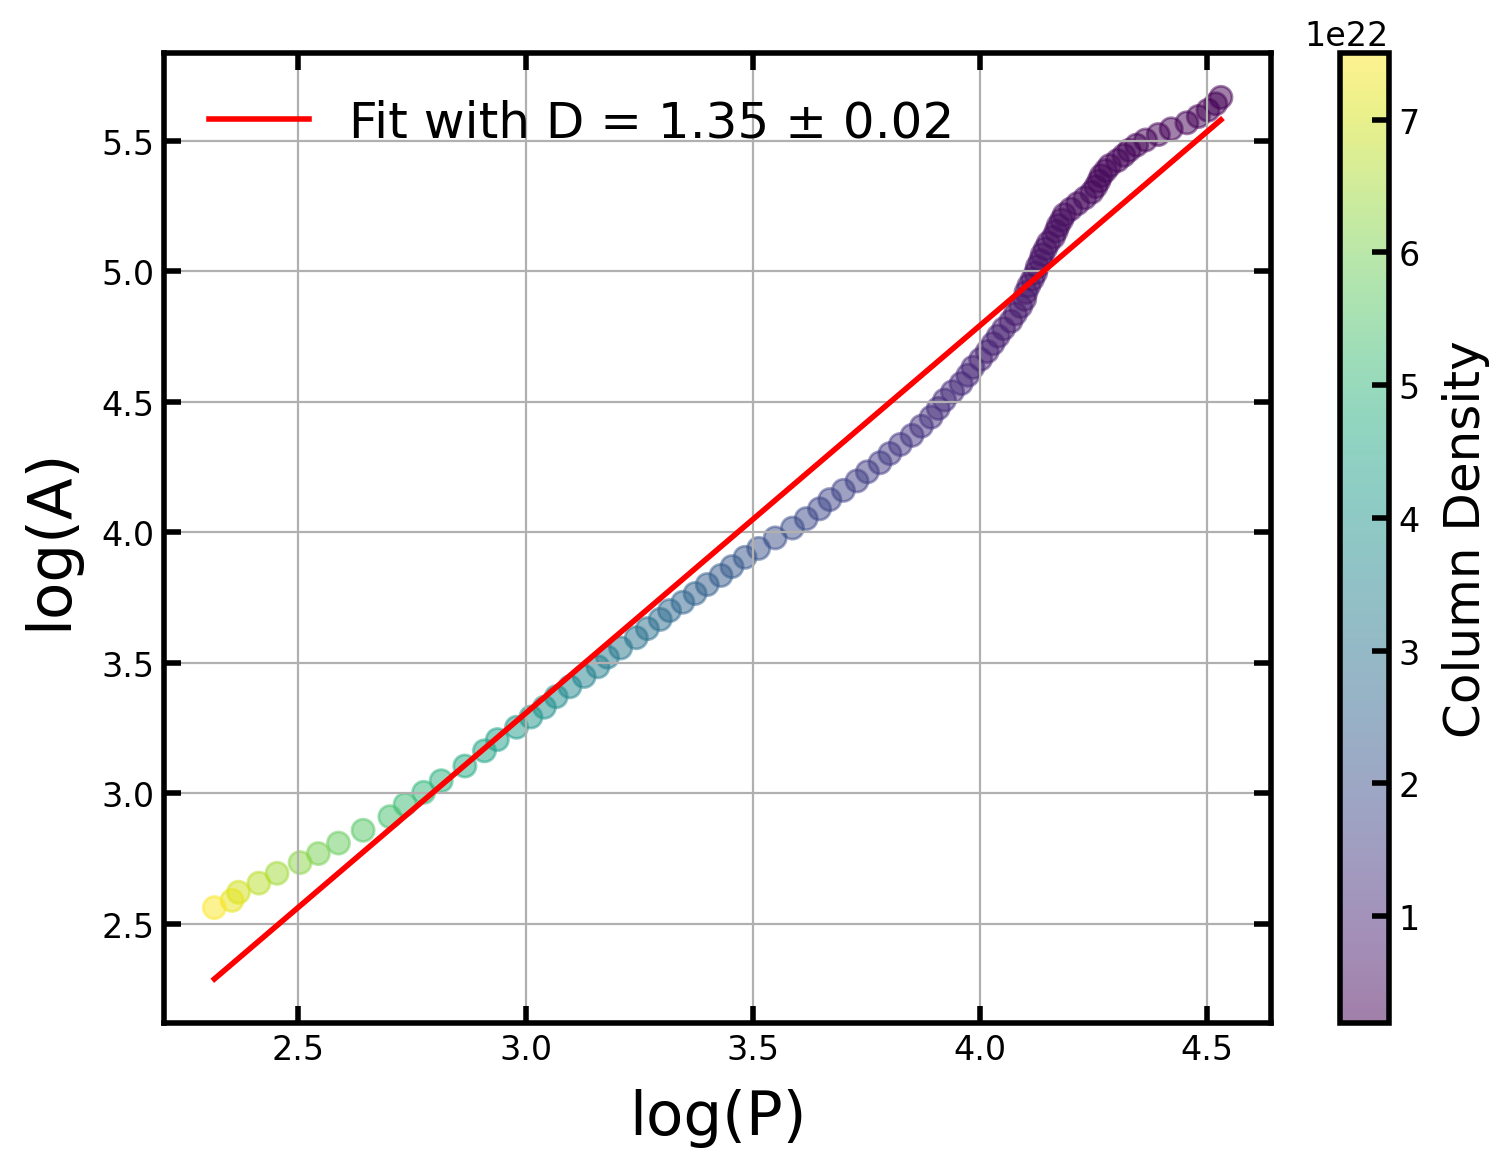
\includegraphics[width=0.5\textwidth]{figures/orion_A_global.png}
    \caption{Perimeter-area relation for Orion A. The solid line indicates the best-fit linear regression in log-log space used to estimate the global fractal dimension \(D_{\mathrm{Global}}\). Residuals are shown in the lower panel.}
    \label{fig:orion_A_global}
\end{figure}

However, the Orion A data show systematic deviations from a single power law across the full column-density range. To account for this, we performed a segmented i.e. double linear fit, dividing the data at \(N = 1.23 \times 10^{22}\,\mathrm{cm}^{-2}\). The two resulting global fractal dimensions from the slopes are:
\[
D_{\mathrm{OA,\,1}} = 1.65 \pm 0.01 \quad \text{(high column density)},
\]
\[
D_{\mathrm{OA,\,2}} = 0.97 \pm 0.3 \quad \text{(low column density)}.
\]
The corresponding mean absolute residuals are 0.0222 (correlation coefficient = 0.9986) for the high-density regime and 0.0679 (correlation coefficient = 0.9748) for the low-density regime, representing a clear improvement compared to the single-fit model.  
Figure \ref{fig:orion_A_global_double_fit} shows the two fitted segments and their residuals. The distinct change in slope suggests a structural transition or the coexistence of different regimes of spatial complexity in Orion A.

\begin{figure}[t]
    \centering
    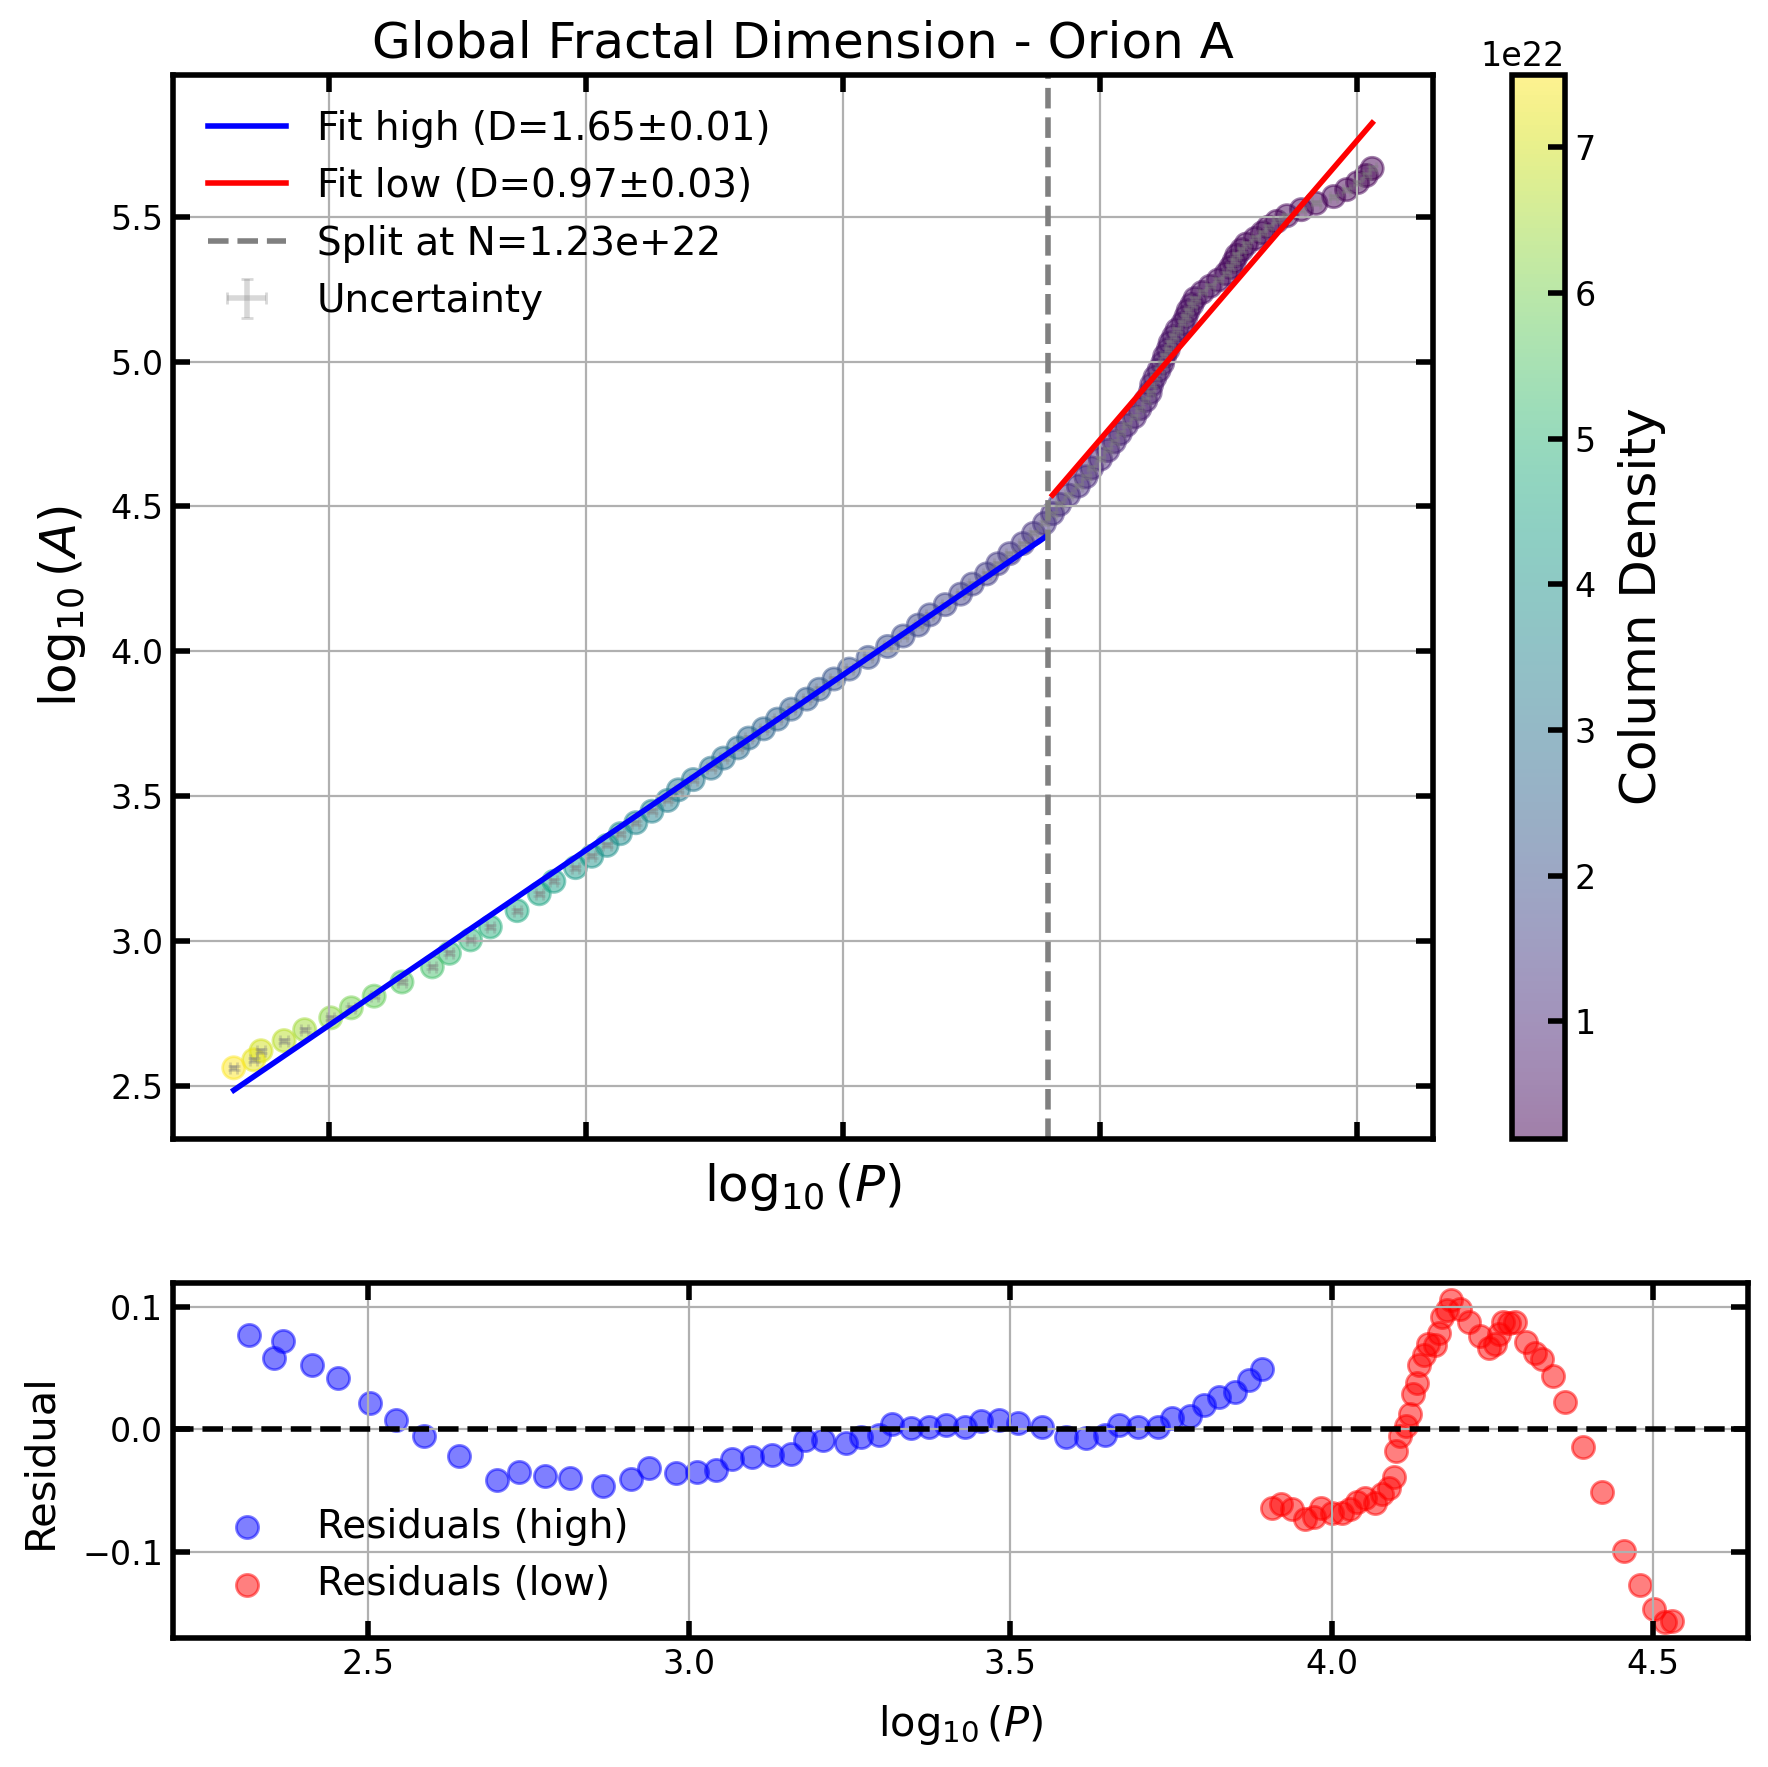
\includegraphics[width=0.5\textwidth]{figures/orion_A_global_double_fit.png}
    \caption{Perimeter-area relation for Orion A with a segmented linear fit. Dashed lines indicate the two fitted regimes, separated at \(N = 1.23 \times 10^{22}\,\mathrm{cm}^{-2}\). Residuals are shown in the lower panel.}
    \label{fig:orion_A_global_double_fit}
\end{figure}

In contrast, Orion B exhibits a well-behaved perimeter-area relation that is accurately described by a single linear fit across the entire column-density range:
\[
D_{\mathrm{OB,\,Global}} = 1.40 \pm 0.01 .
\]
The corresponding residuals (mean absolute residual = 0.0493) and correlation coefficient (0.9976) confirm the robustness of this fit. Figure \ref{fig:orion_B_global} shows the fitted relation and residuals. The consistency of the slope across scales indicates a more uniform degree of structural complexity compared to Orion~A.

\begin{figure}[t]
    \centering
    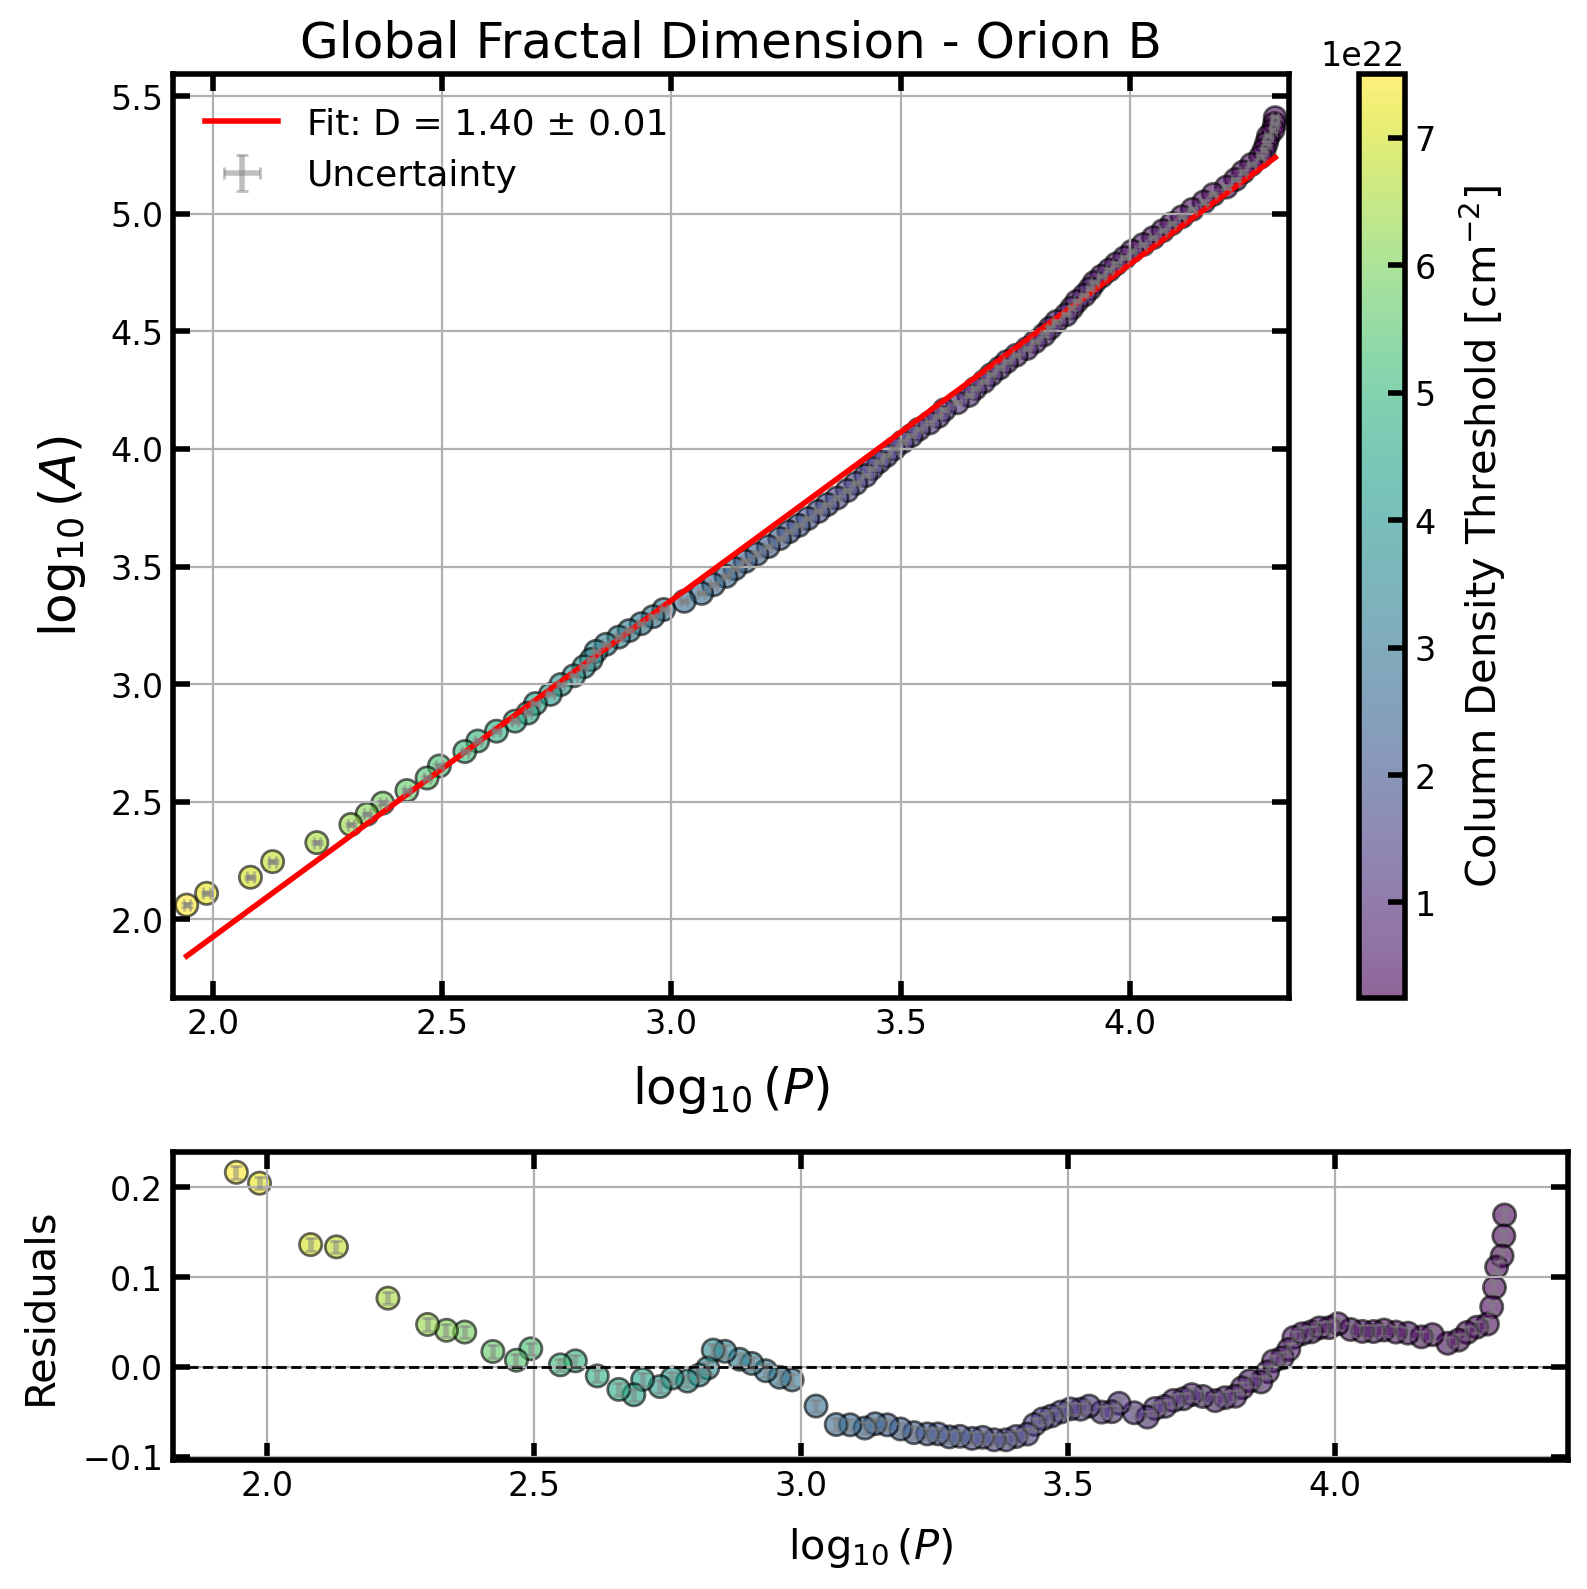
\includegraphics[width=0.5\textwidth]{figures/orion_B_global.png}
    \caption{Perimeter-area relation for Orion~B with the best-fit linear regression overlaid. Residuals are shown in the lower panel.}
    \label{fig:orion_B_global}
\end{figure}

The uncertainties in perimeter and area measurements were estimated at 1.6\%, based on simulations demonstrating that this level of error is representative across different reference geometries.

\section{Local Properties}

\subsection{Euler Characteristic}

We evaluated the Euler characteristic, \(\chi\), for both Orion A and Orion B as a function of the column–density threshold. This topological descriptor quantifies the connectivity and fragmentation of structures within the clouds: negative values of \(\chi\) indicate a predominance of isolated regions, while more positive values reflect a higher degree of connectivity.

Figures~\ref{fig:Euler_Orion_A_no_figs} and~\ref{fig:Euler_Orion_B_no_figs} present the results for Orion A and Orion B, respectively. In both cases of Orion A and B, \(\chi\) was computed over the same range of column densities \(N_\mathrm{min} \leq N \leq N_\mathrm{max}\) used in the gloabl perimeter–area analysis above, ensuring consistency and comparability.

\begin{figure}[t]
    \centering
    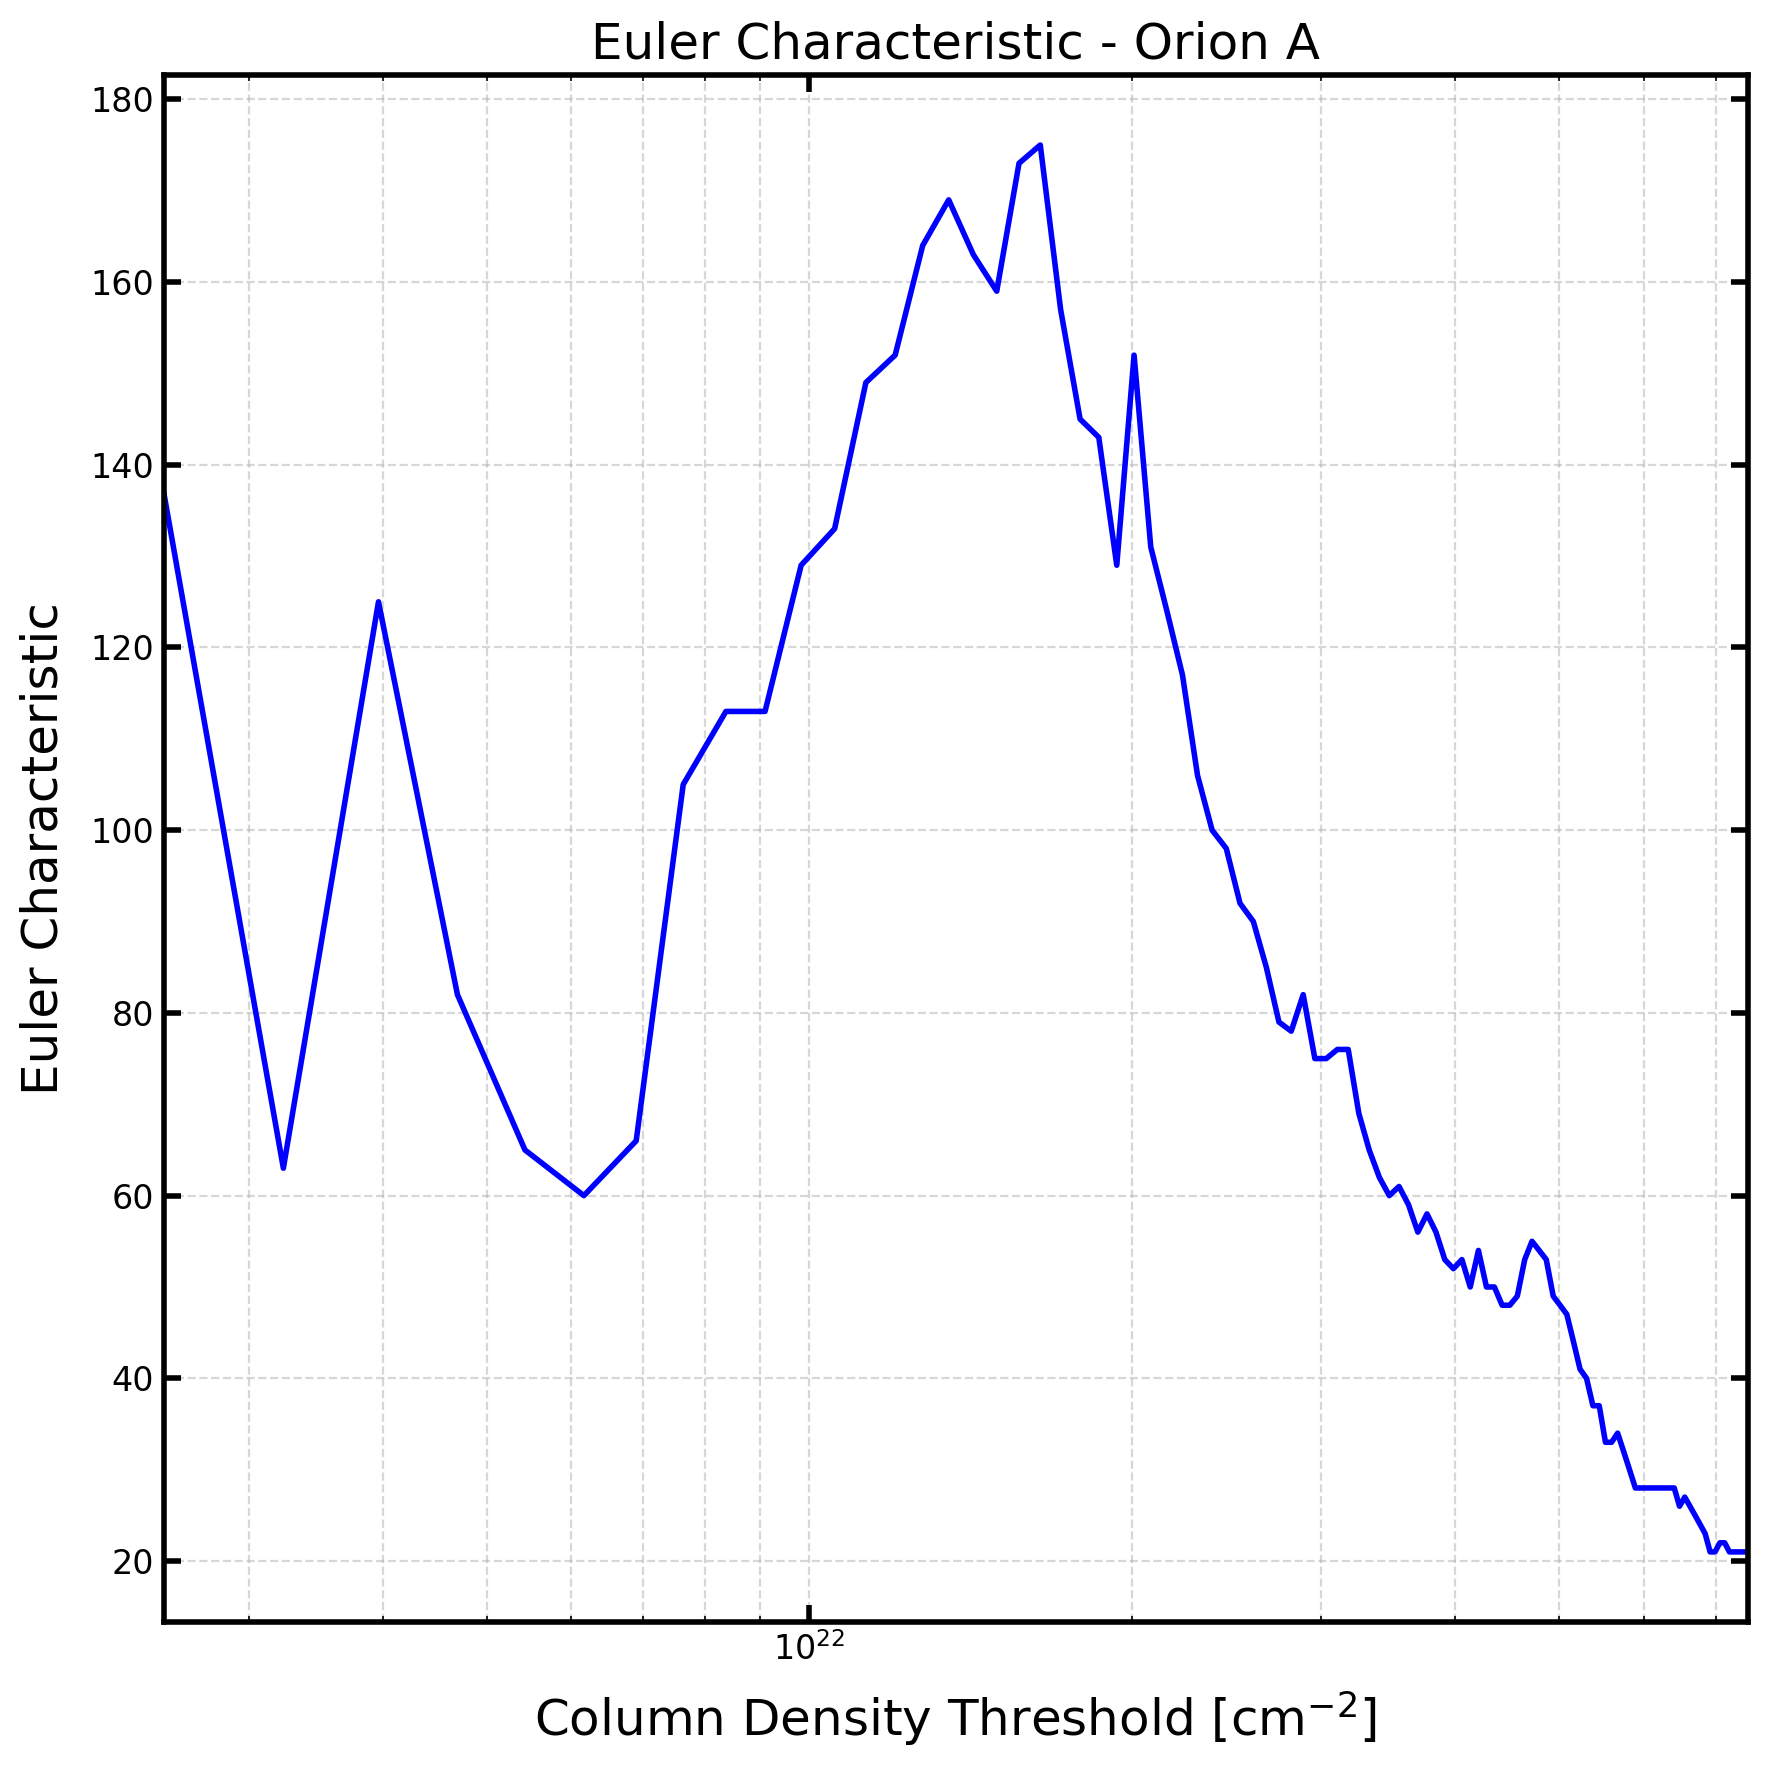
\includegraphics[width=0.45\textwidth]{figures/euler_Orion_A_no_figs.png}
    \caption{Euler characteristic of Orion A as a function of column–density threshold. Positive values correspond to a predominance of isolated structures, while negative values indicate higher connectivity.}
    \label{fig:Euler_Orion_A_no_figs}
\end{figure}

\begin{figure}[t]
    \centering
    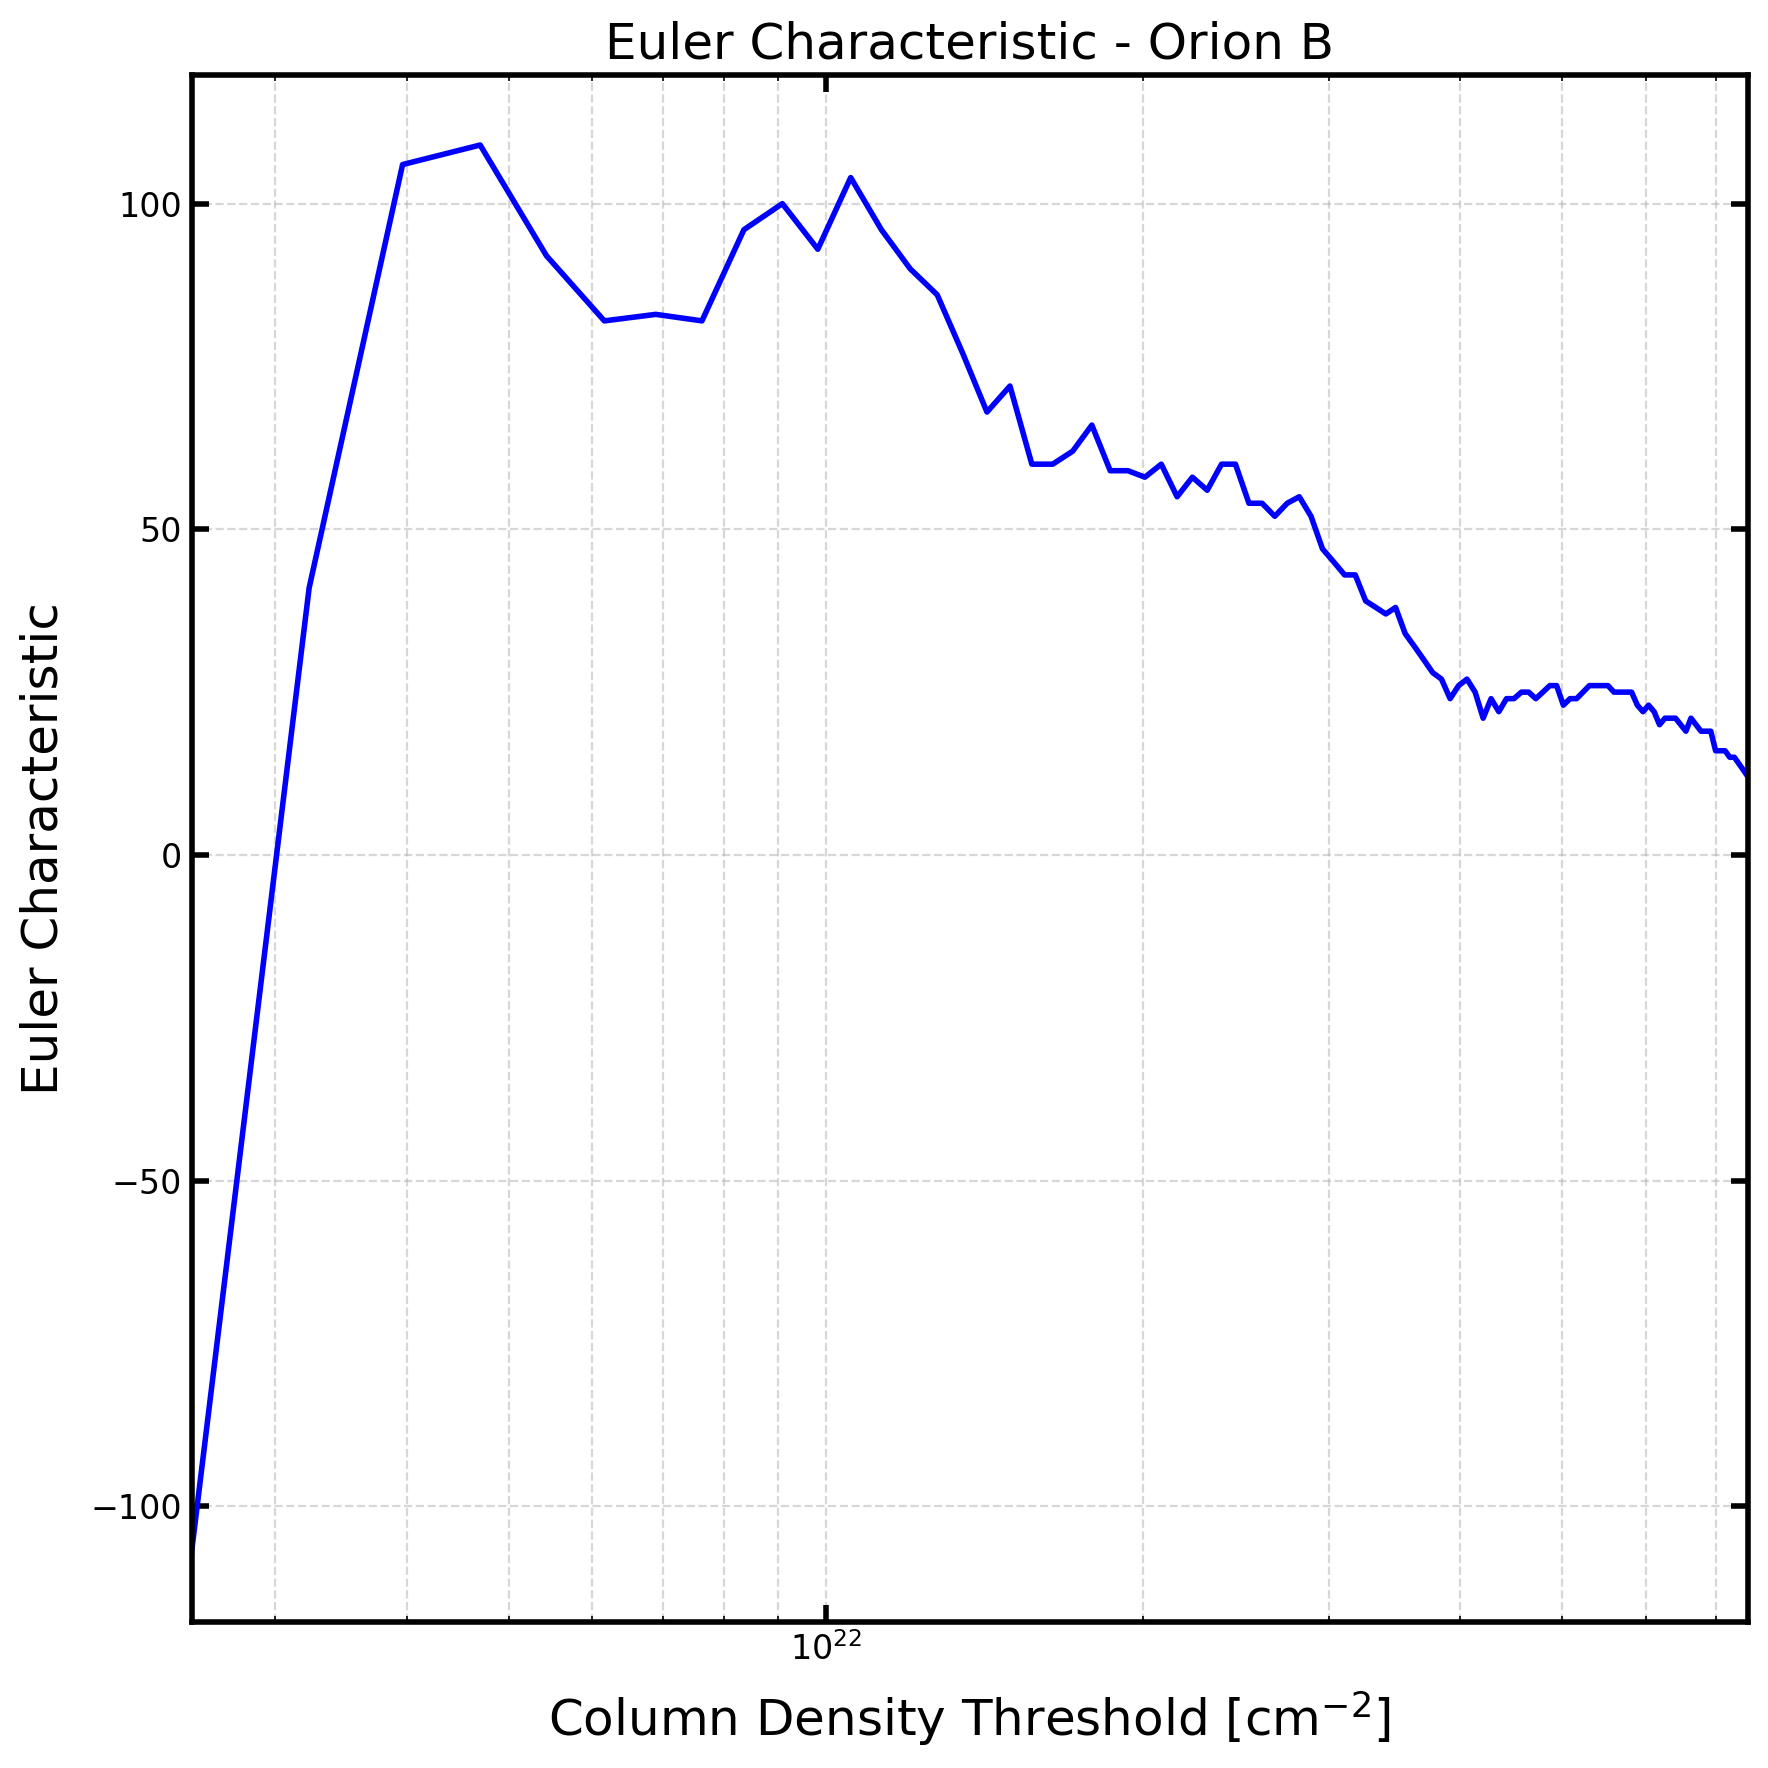
\includegraphics[width=0.45\textwidth]{figures/euler_Orion_B_no_figs.png}
    \caption{Euler characteristic of Orion~B as a function of column–density threshold.}
    \label{fig:Euler_Orion_B_no_figs}
\end{figure}

Orion A exhibits a profile that closely resembles the Gaussian‑like behavior expected from Gaussian Random Field simulations (Figure \ref{fig:sims_euler_char}), with a pronounced peak at approximately $1.64 \times 10^{22} \,\mathrm{cm}^{-2}$. In contrast, Orion B shows a more linear trend. In both regions, strong numerical fluctuations appear at lower column-density thresholds, leading to noticeable variations in the calculated Euler characteristic.

\subsection{Local Fractal Dimension}

Figure~\ref{fig:local_Orion_A_B} shows the variation of the local fractal dimension $D(\nu)$ as a function of column-density threshold for Orion A and Orion B. The column density range  \(N_\mathrm{min} \leq N \leq N_\mathrm{max}\) is the same as in the previous sections. In both regions we find a clear overall trend: the local fractal dimension changes systematically as the threshold increases. Superimposed on this trend, several pronounced peaks and deviations are visible. These features likely trace transitions in the morphology of the structures, for instance the emergence of compact cores or the fragmentation of filaments into smaller substructures.

A more detailed interpretation of these peaks and their implications for cloud evolution and turbulence will be addressed in the following section.

\begin{figure}[t]
    \centering
    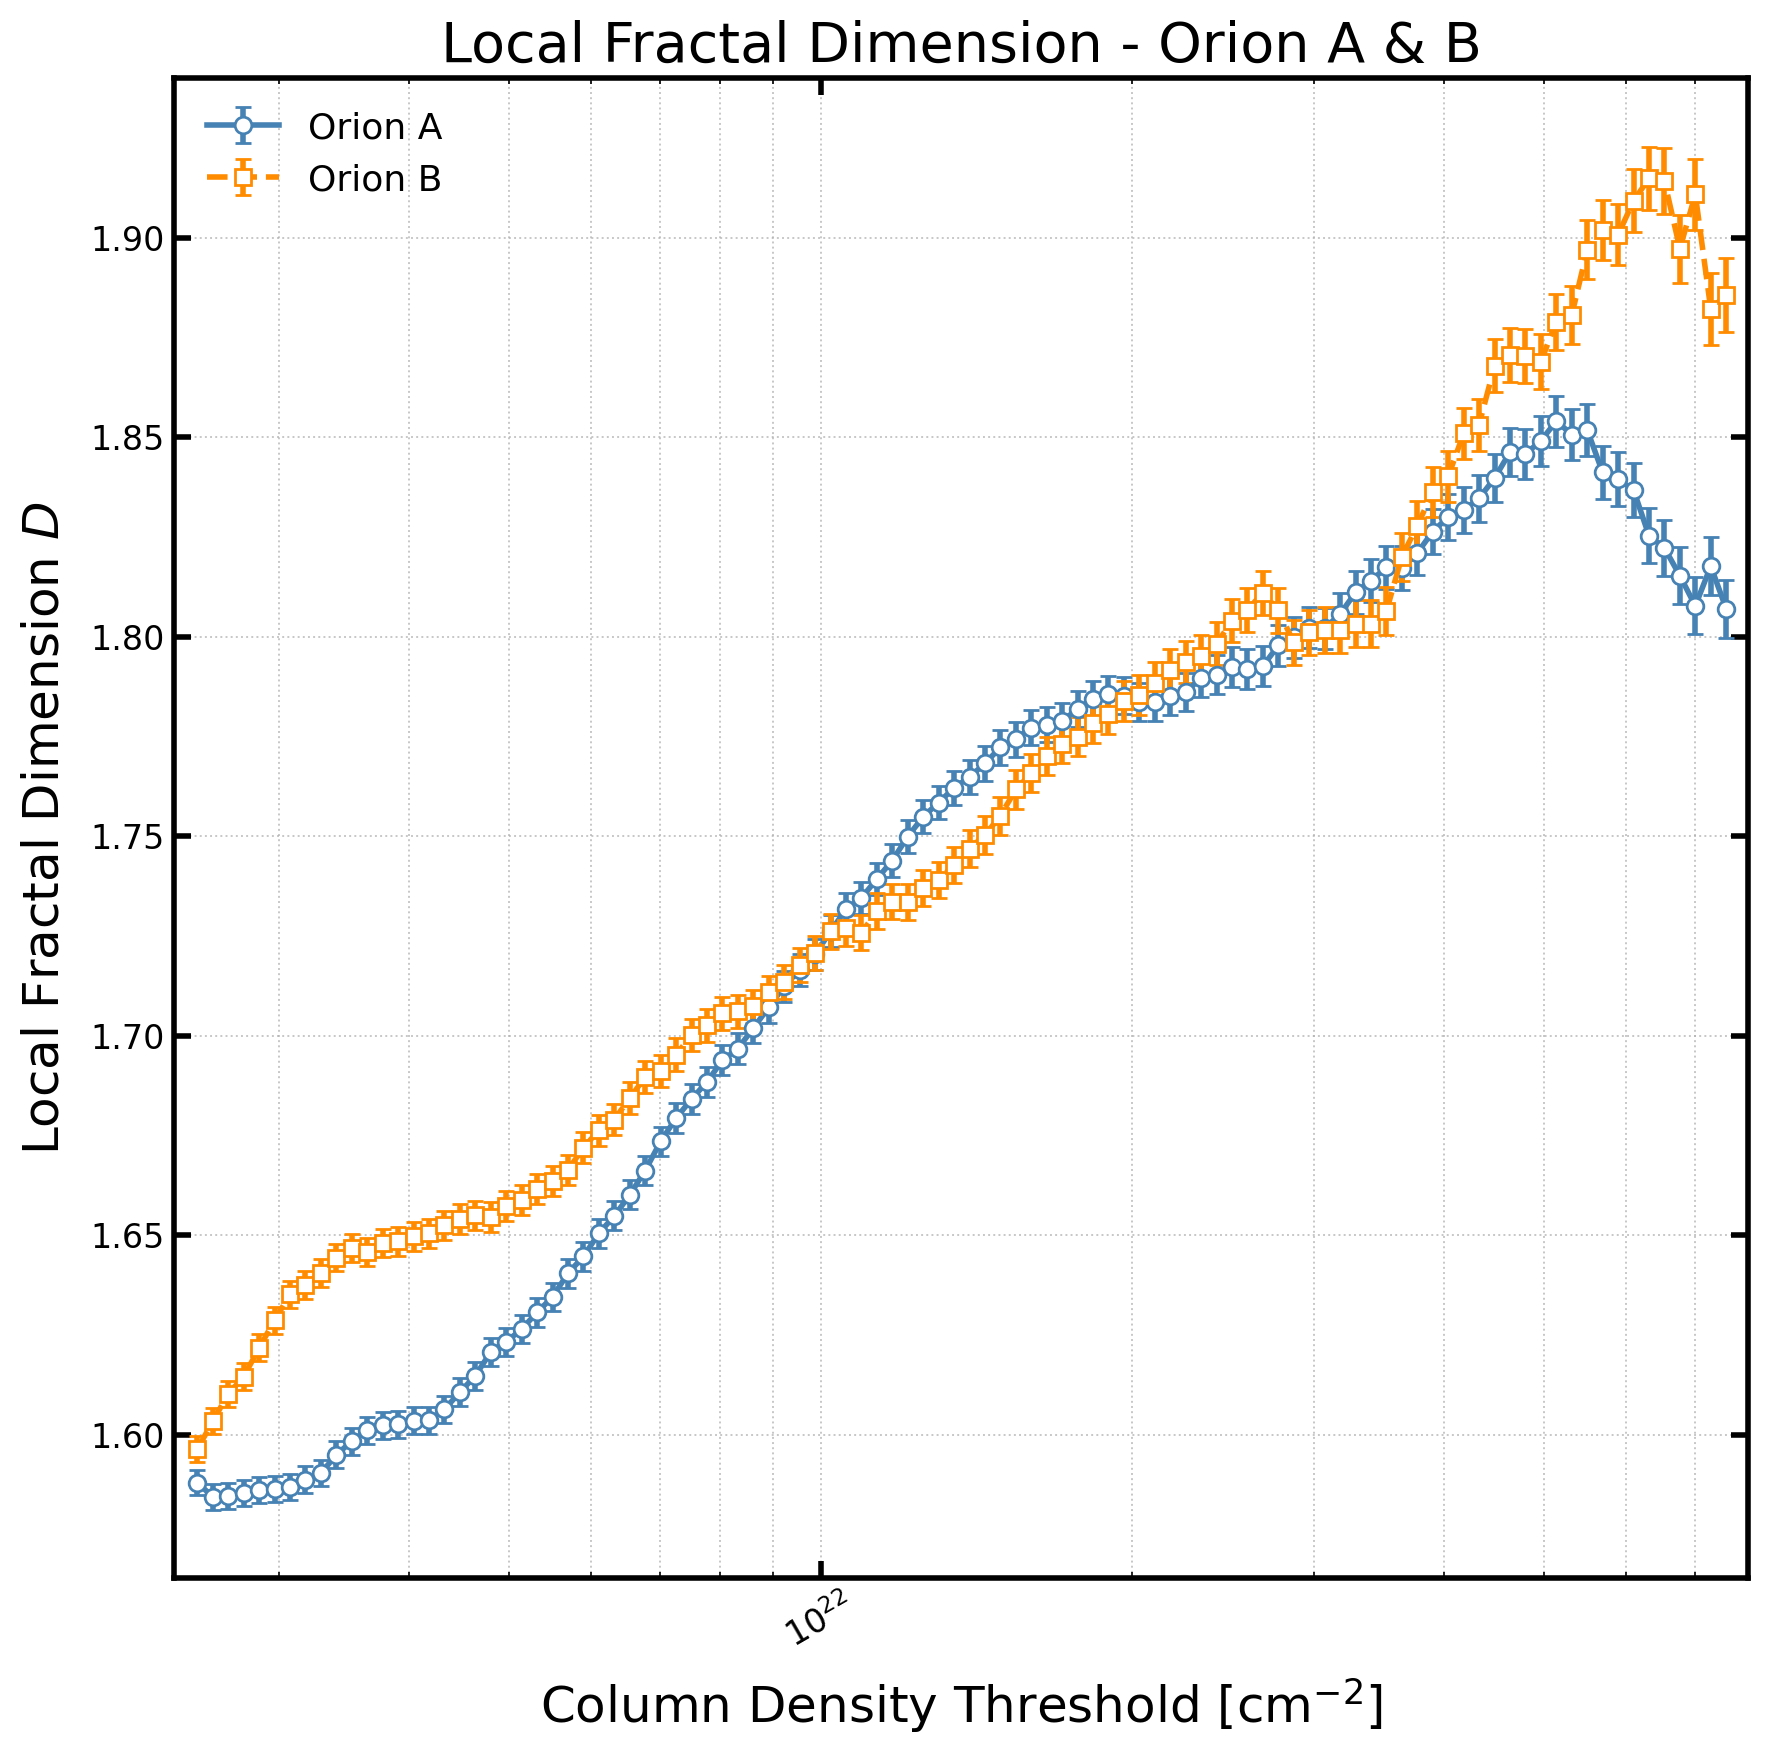
\includegraphics[width=0.5\textwidth]{figures/local_orion_A_B.png}
    \caption{Local fractal dimension as a function of column-density threshold for Orion A and Orion B. Error bars reflect the uncertainties of the fit at each threshold.}
    \label{fig:local_Orion_A_B}
\end{figure}

The average values and their standard deviations of the local fractal dimension for the two regions are:
\[
\bar{D}_{\mathrm{OA,\,Local}} = 1.73 \pm 0.09,
\]
\[
\bar{D}_{\mathrm{OB,\,Local}} = 1.75 \pm 0.08.
\]

The uncertainties in perimeter and area measurements were estimated again at approximately 1.6\%, based on simulation results.

% To-Do:
% add uncertainties
% make graphs more similar to local Orion A and B
% add average values 
\subsection{Analysis of Individual Structures}

To gain deeper insight into the fractal properties of each cloud, we decomposed the emission at every column-density threshold into its set of connected structures. This dendrogram-based approach provides a hierarchical view of how the material is organized into nested substructures, enabling a more detailed examination of their geometrical and topological properties.

Figures~\ref{fig:dendrogram_A} and~\ref{fig:dendrogram_B} display the resulting dendrograms for Orion~A and Orion~B. These diagrams trace how individual regions merge into larger complexes as the threshold decreases, effectively capturing the clustering behaviour of the cloud across spatial scales.

\begin{figure}[t]
    \centering
    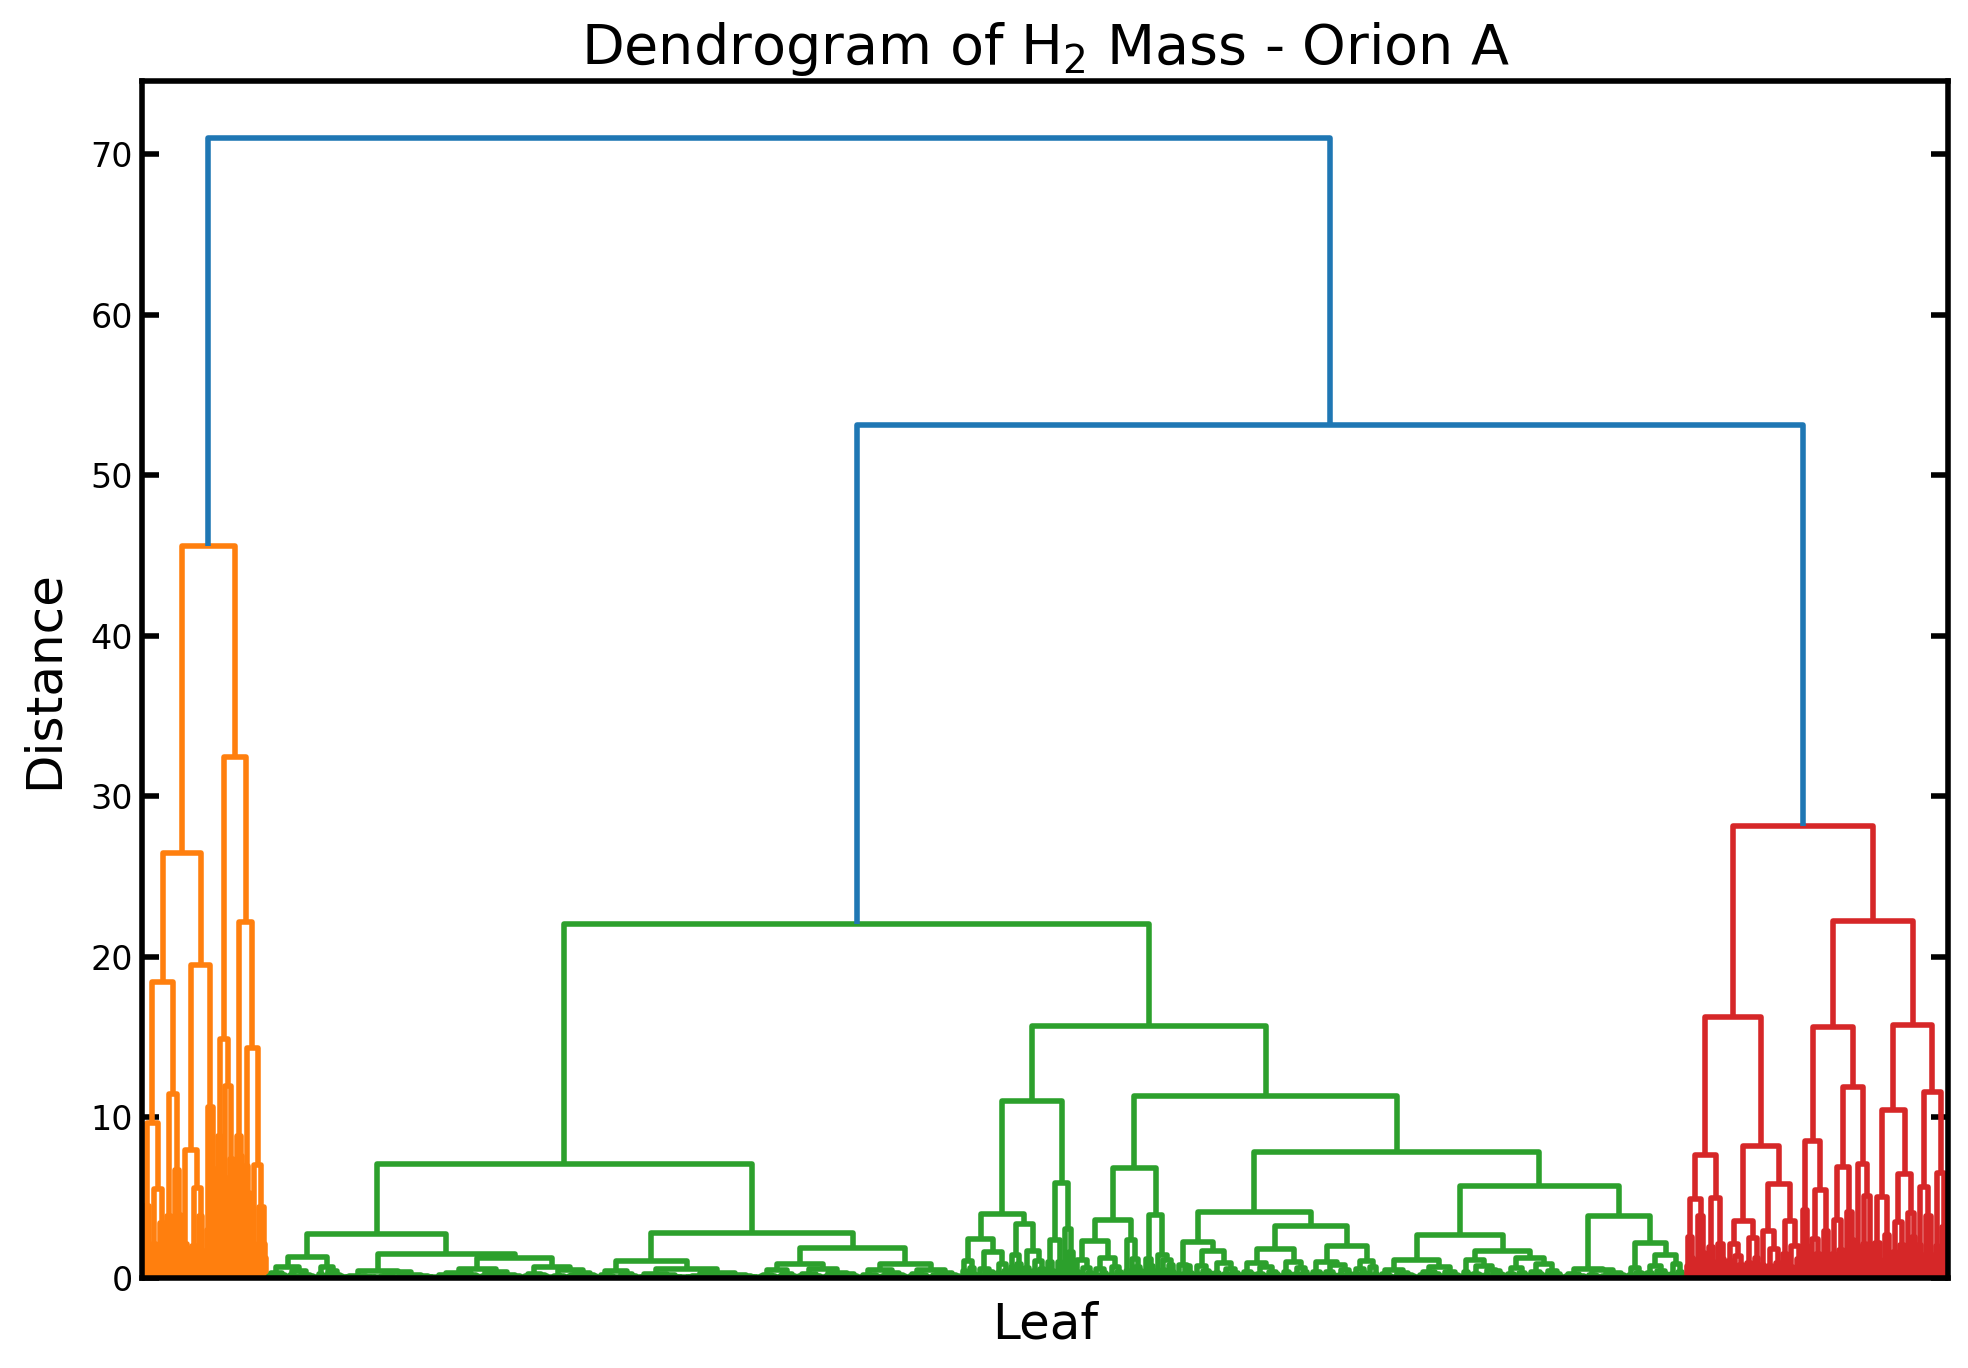
\includegraphics[width=0.5\textwidth]{figures/dendogram_A.png}
    \caption{Dendrogram of the Orion~A mass distribution, showing the hierarchical merging of structures as the column-density threshold is lowered. The various main branches are coloured differently for highlighting purposes. The y-axis "Distance" represents a degree of similarity between structures. }
    \label{fig:dendrogram_A}
\end{figure}

\begin{figure}[t]
    \centering
    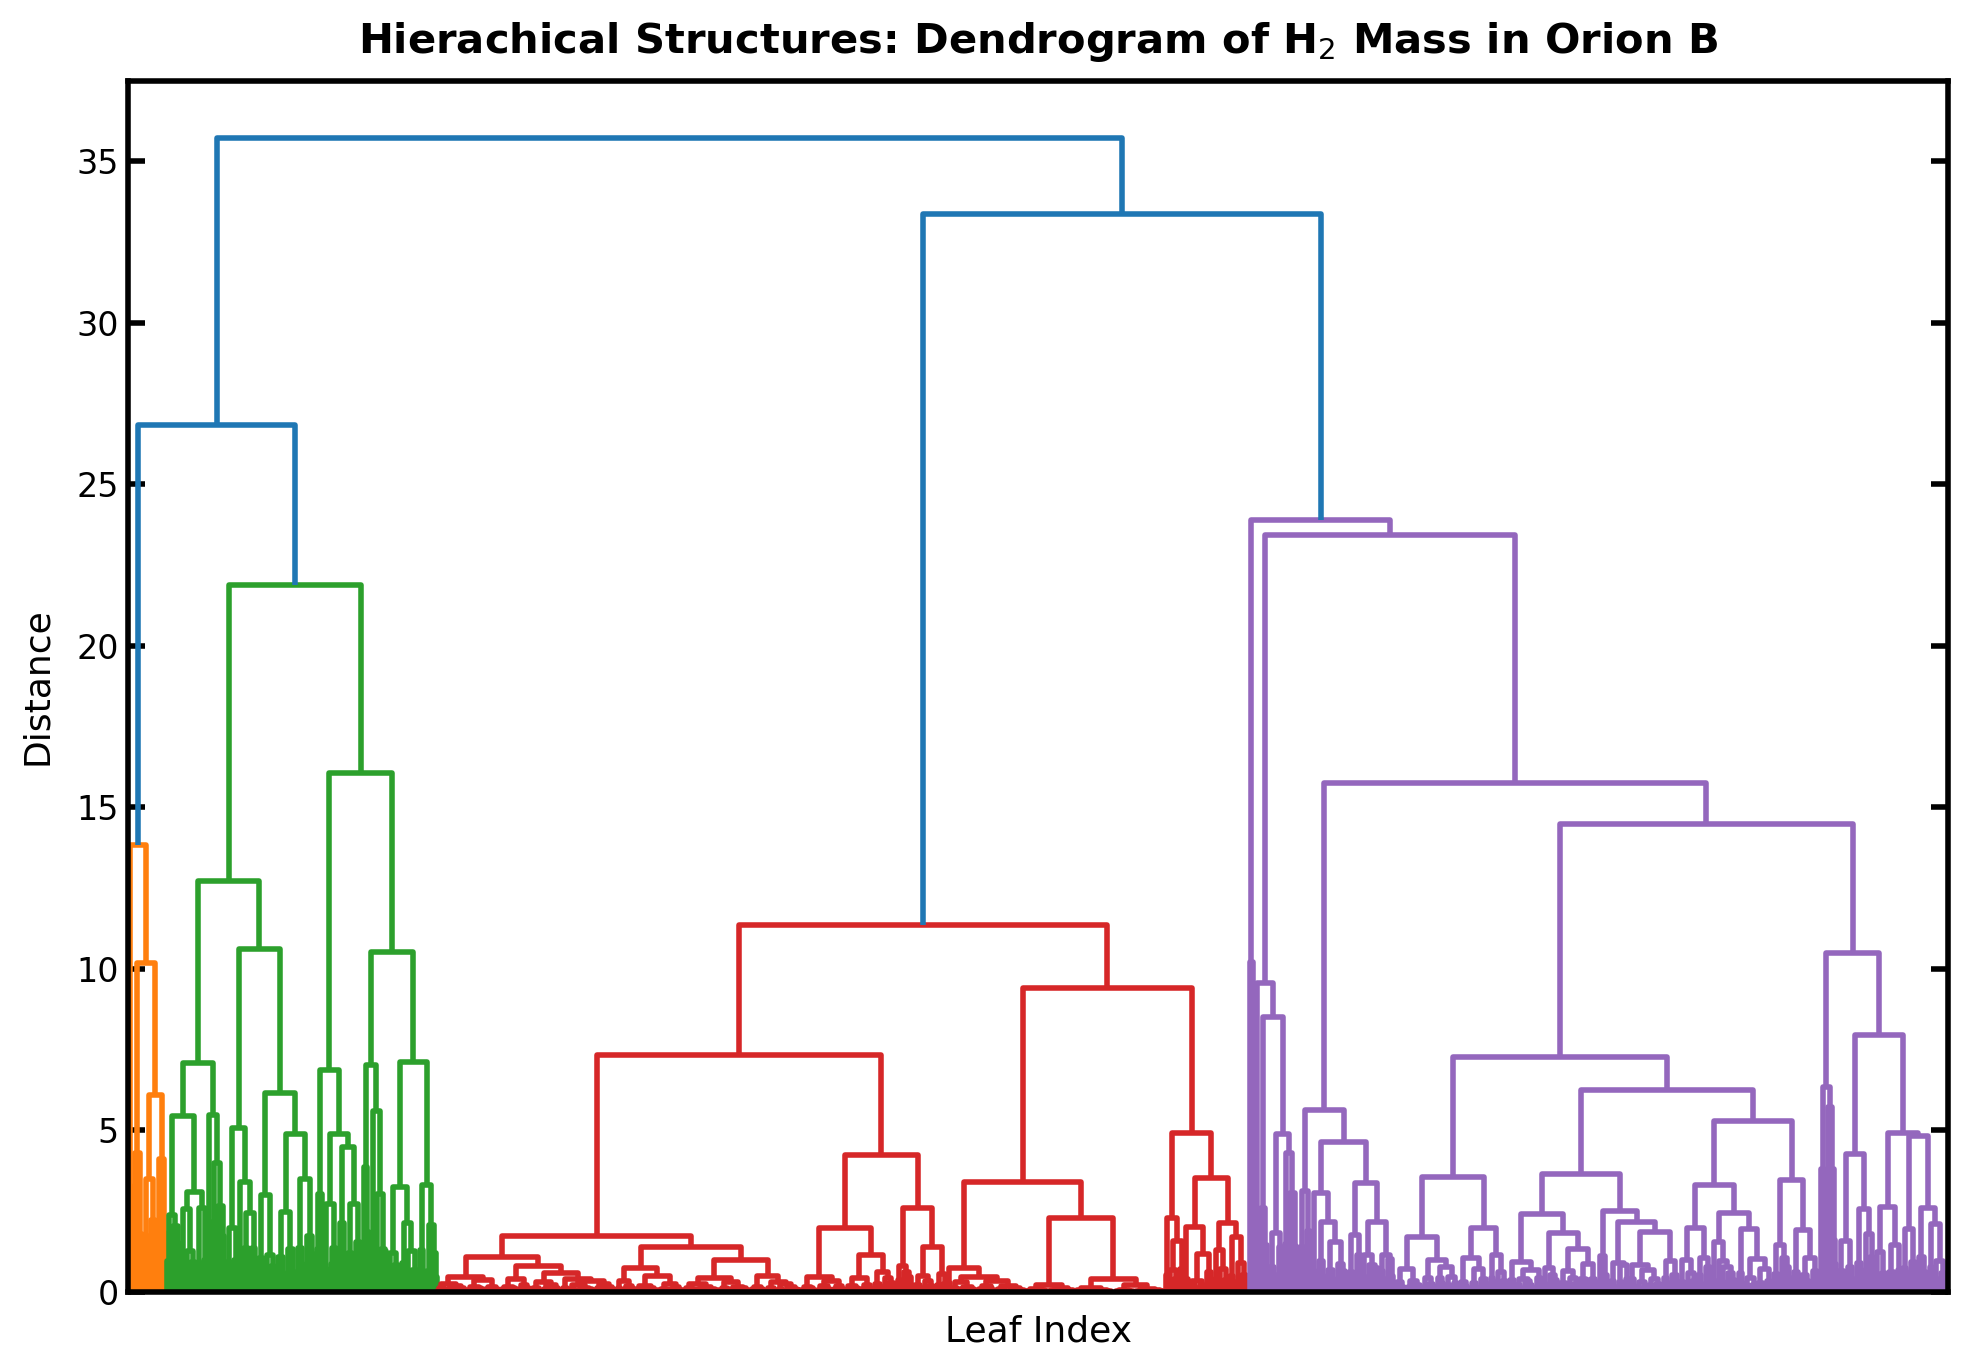
\includegraphics[width=0.5\textwidth]{figures/dendogram_B.png}
    \caption{Dendrogram of the Orion~B mass distribution, showing the hierarchical merging of structures as the column-density threshold is lowered.}
    \label{fig:dendrogram_B}
\end{figure}

We then applied the same calculation of the local fractal dimension to each of these connected structures. For numerical stability, we first limited the analysis to the largest regions at each threshold, selecting them according to minimum perimeter and area criteria. The resulting measurements are shown in Figures~\ref{fig:local_A_single_structures} and~\ref{fig:local_B_single_structures}. Overall, these individual-structure analyses reproduce similar trends to those found in the undifferentiated calculation (Figure~\ref{fig:local_Orion_A_B}), although with shallower progression at higher column density thresholds. 
This behaviour has been recorded in other instances, e.g. when the regions got simply divided into N sharp cuts: the calculated local fractal dimensions show similar trends, but with a shallower progression. The average of these then tends to approach the whole region one.   

\begin{figure}[t]
    \centering
    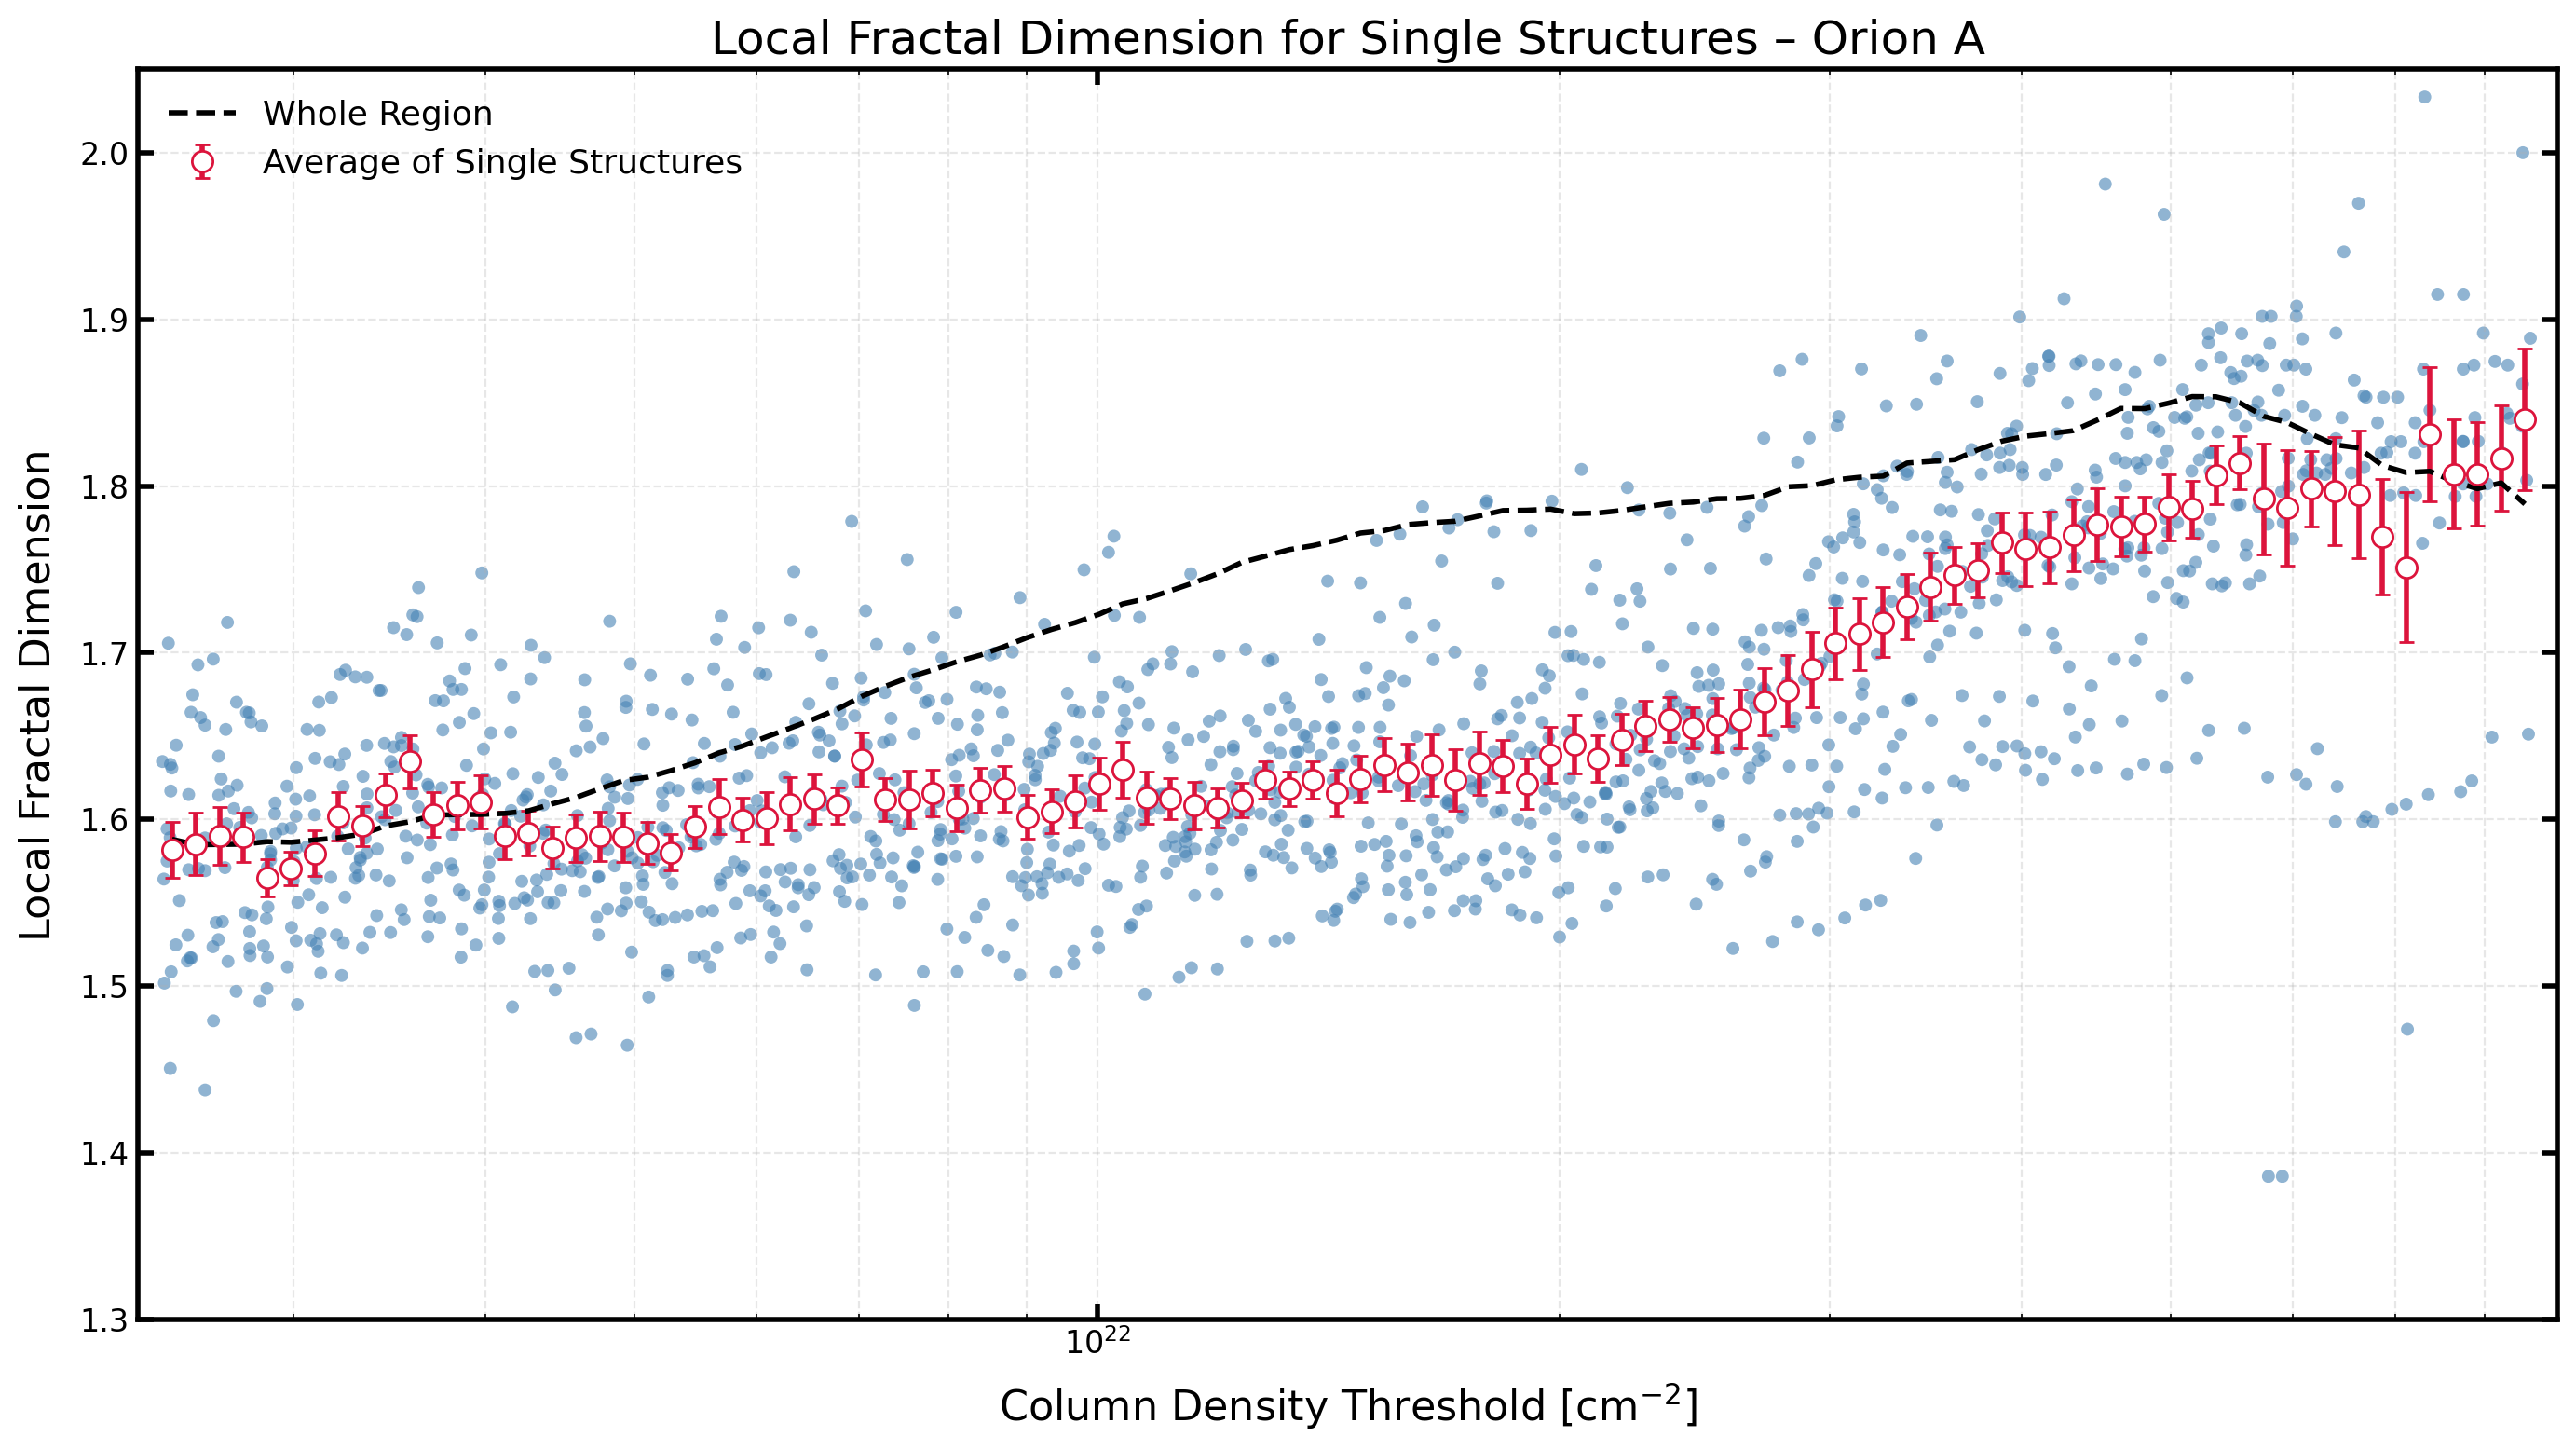
\includegraphics[width=0.75\textwidth]{figures/local_Orion_A_single_structures.png}
    \caption{Local fractal dimension for individual structures in Orion~A as a function of column--density threshold. 
    Shown are the mean values obtained from the largest structures at each threshold (with uncertainties), overlaid with the corresponding values from the undifferentiated calculation.}
    \label{fig:local_A_single_structures}
\end{figure}

\begin{figure}[t]
    \centering
    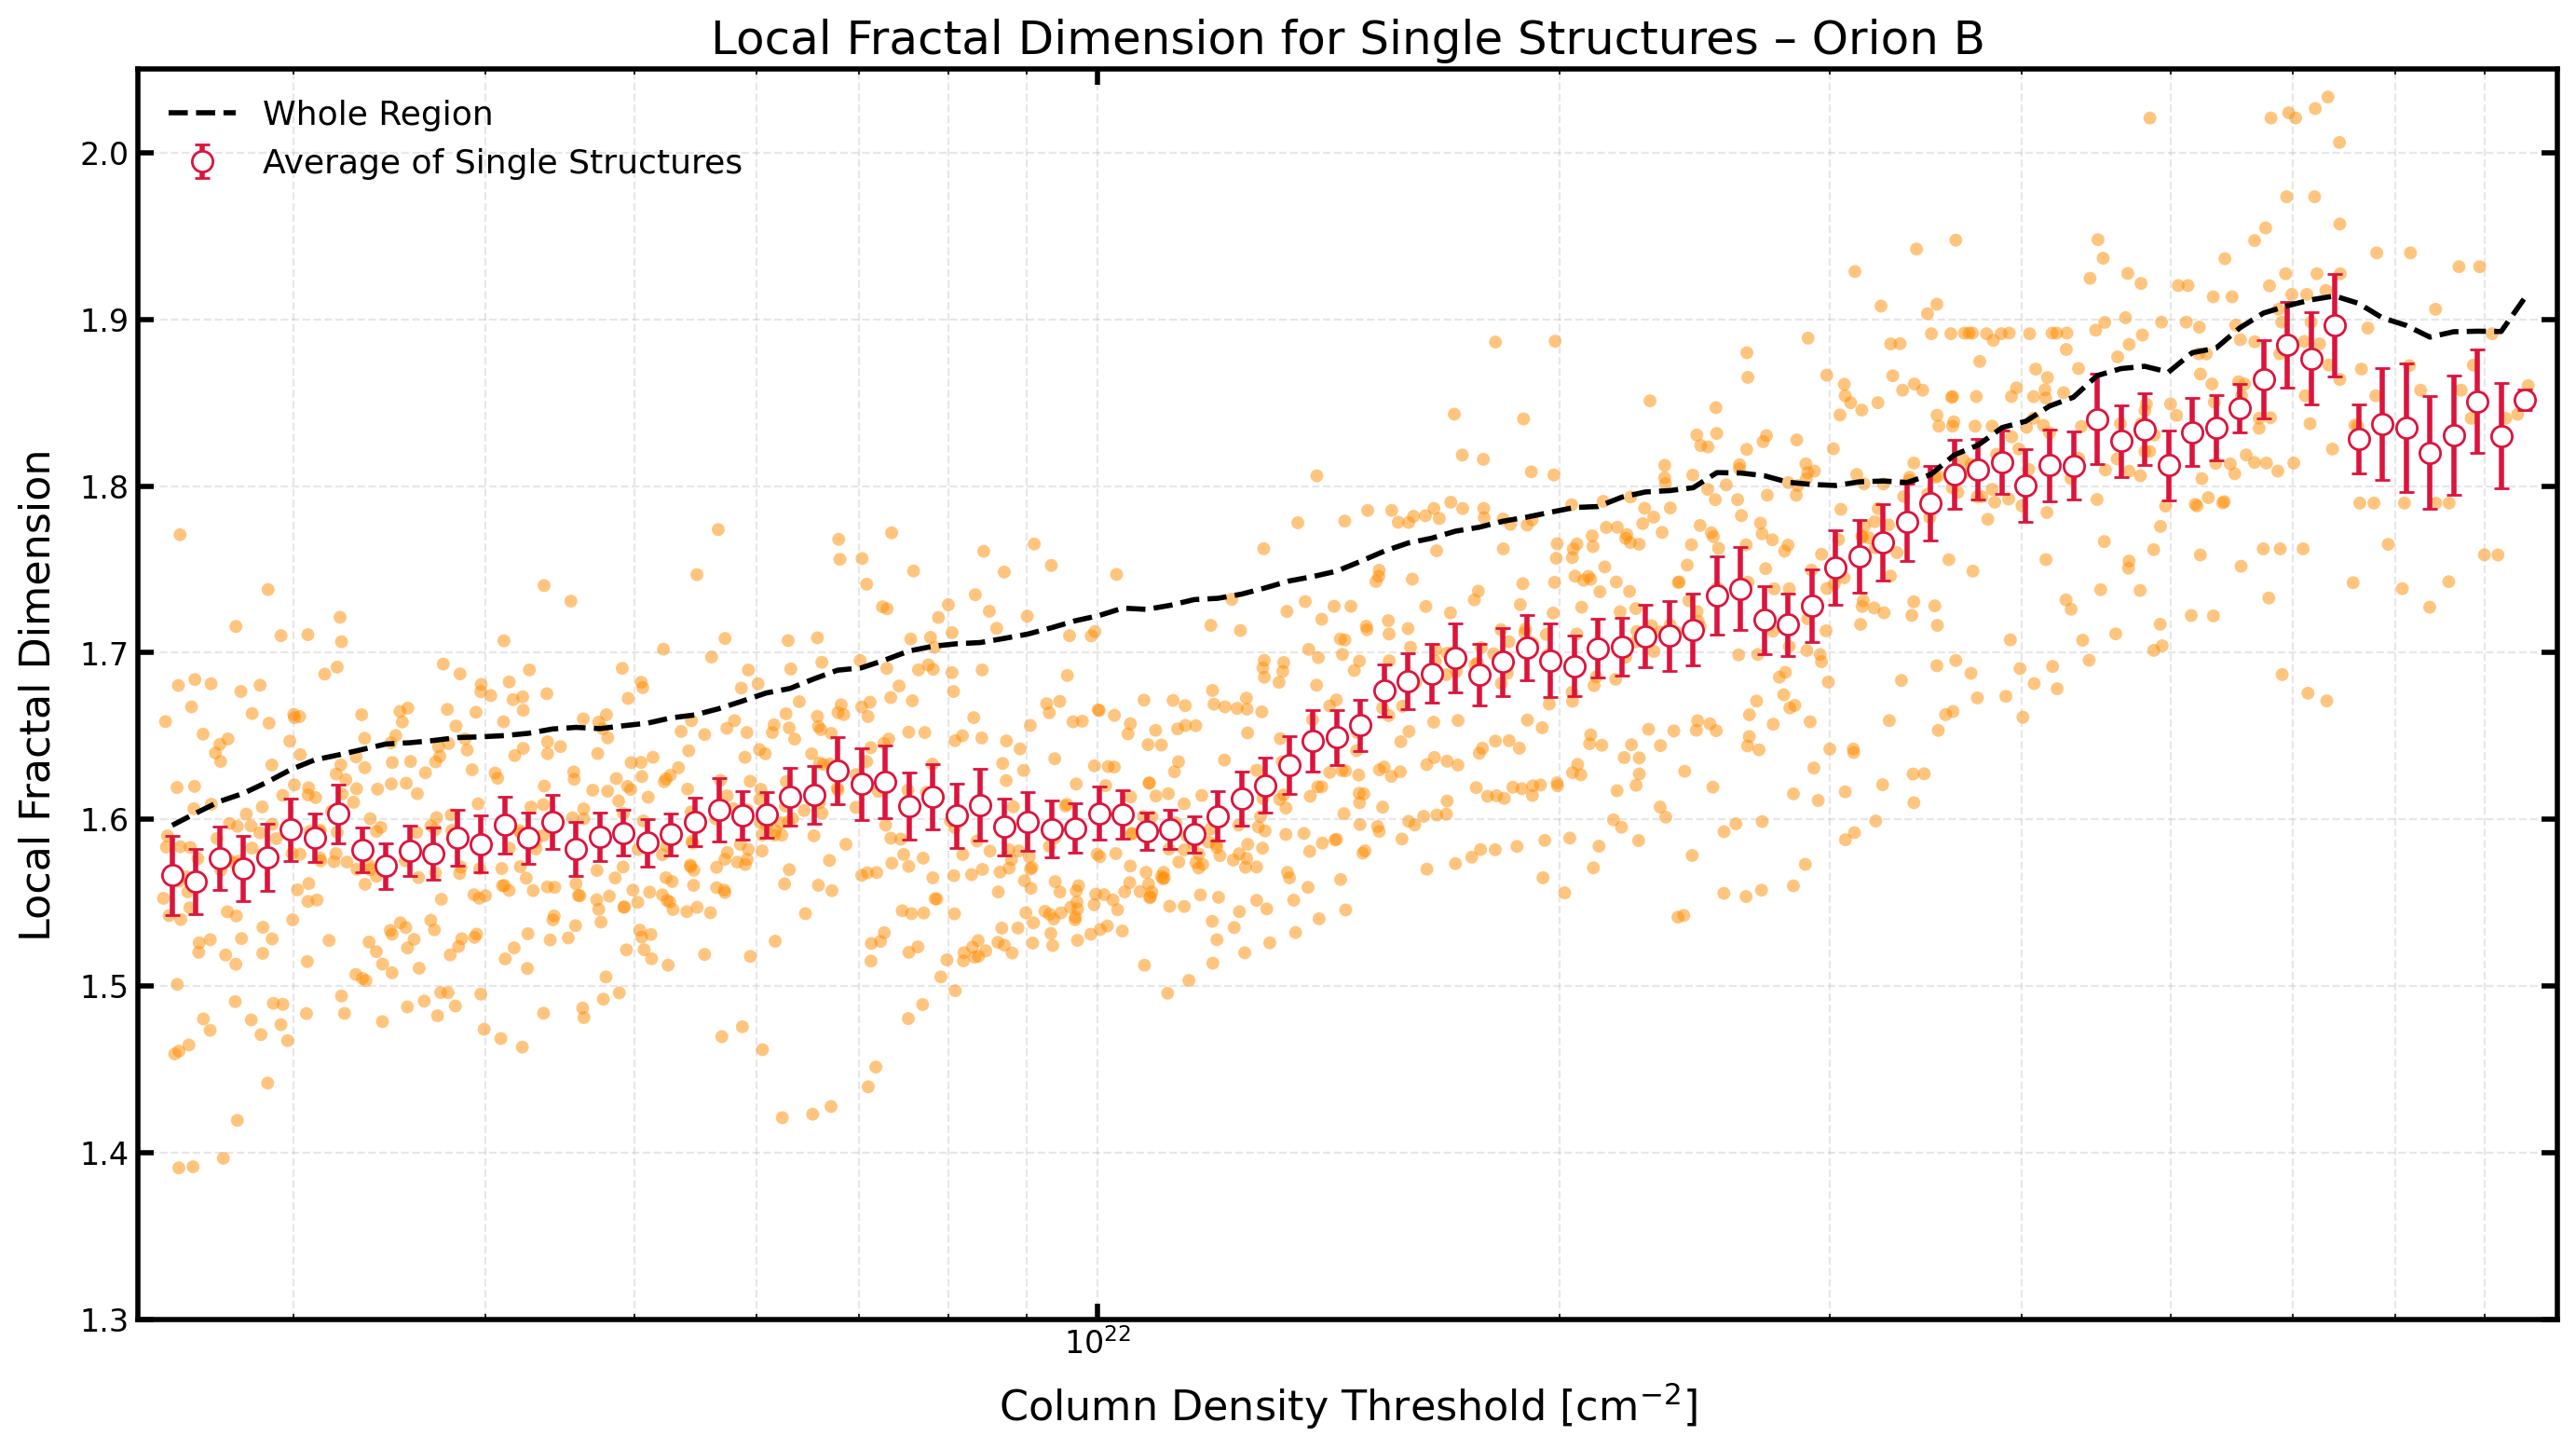
\includegraphics[width=0.75\textwidth]{figures/local_Orion_B_single_structures.png}
    \caption{Local fractal dimension for individual structures in Orion~B as a function of column--density threshold. 
    As in Orion~A, the mean values from the selected structures (with uncertainties) are overlaid with the results from the undifferentiated calculation.}
    \label{fig:local_B_single_structures}
\end{figure}

\subsection{MSD Plane}

To investigate how the fractal properties relate to the physical characteristics of the cloud, we computed the mass, size, and local fractal dimension for each connected structure identified at every column-density threshold in the dendrogram hierarchy.  
These quantities were then plotted against each other, with the local fractal dimension encoded as color.  

The resulting Mass-Size-Fractal Dimension (MSD) planes are shown in Figure \ref{fig:MSD_orion_A} for Orion~A, Figure~\ref{fig:MSD_orion_B} for Orion~B, and Figure~\ref{fig:MSD_orion_A_B} for the combined dataset.  
For reference, the expected scaling relations for idealized filamentary structures (\(A = 10\)) and spherical structures (\(A = 3\)) are overplotted, as done in \cite{Hacar_2025}.

\begin{figure}[t]
    \centering
    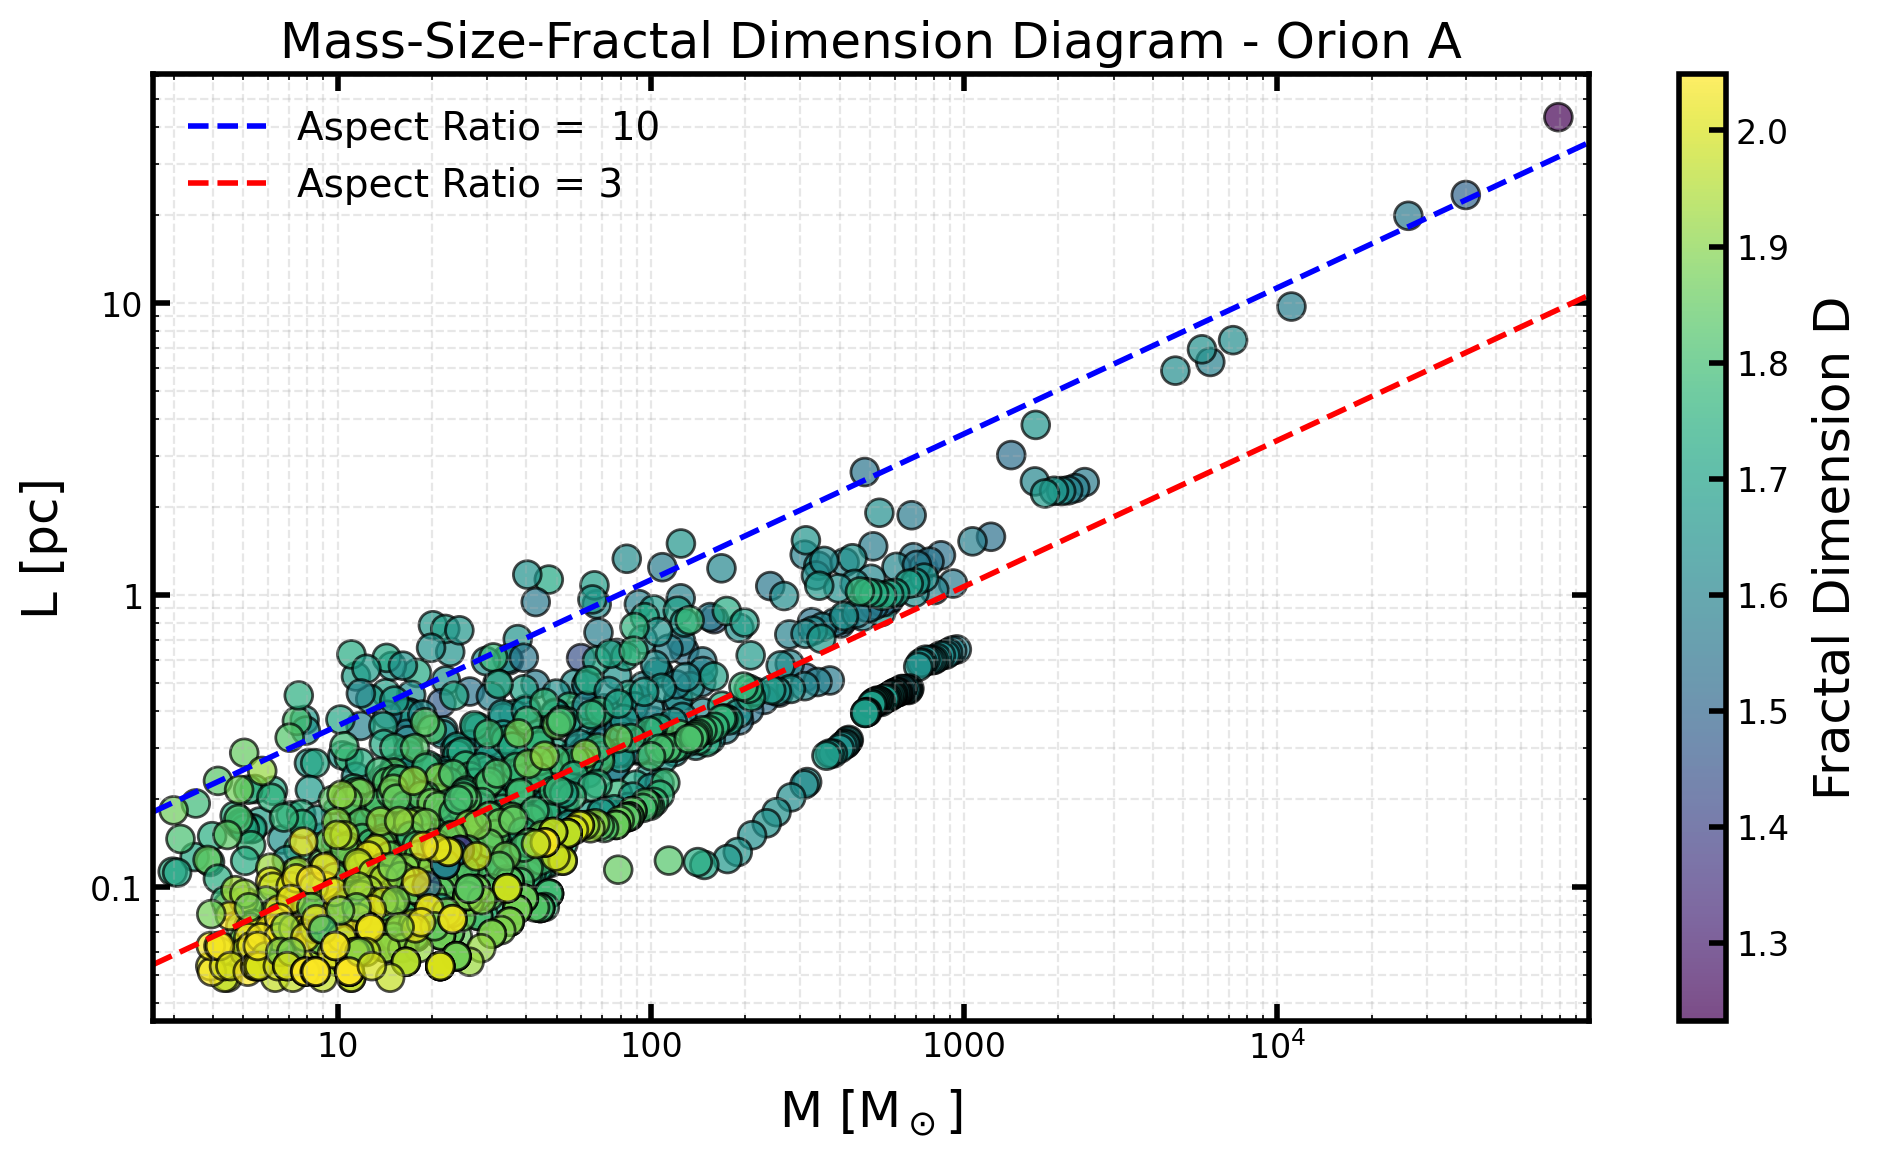
\includegraphics[width=0.6\textwidth]{figures/MSD_Orion_A.png}
    \caption{MSD plane for Orion~A. The color scale indicates the local fractal dimension, and reference scalings for filamentary and spherical geometries are shown as solid lines.}
    \label{fig:MSD_orion_A}
\end{figure}

\begin{figure}[t]
    \centering
    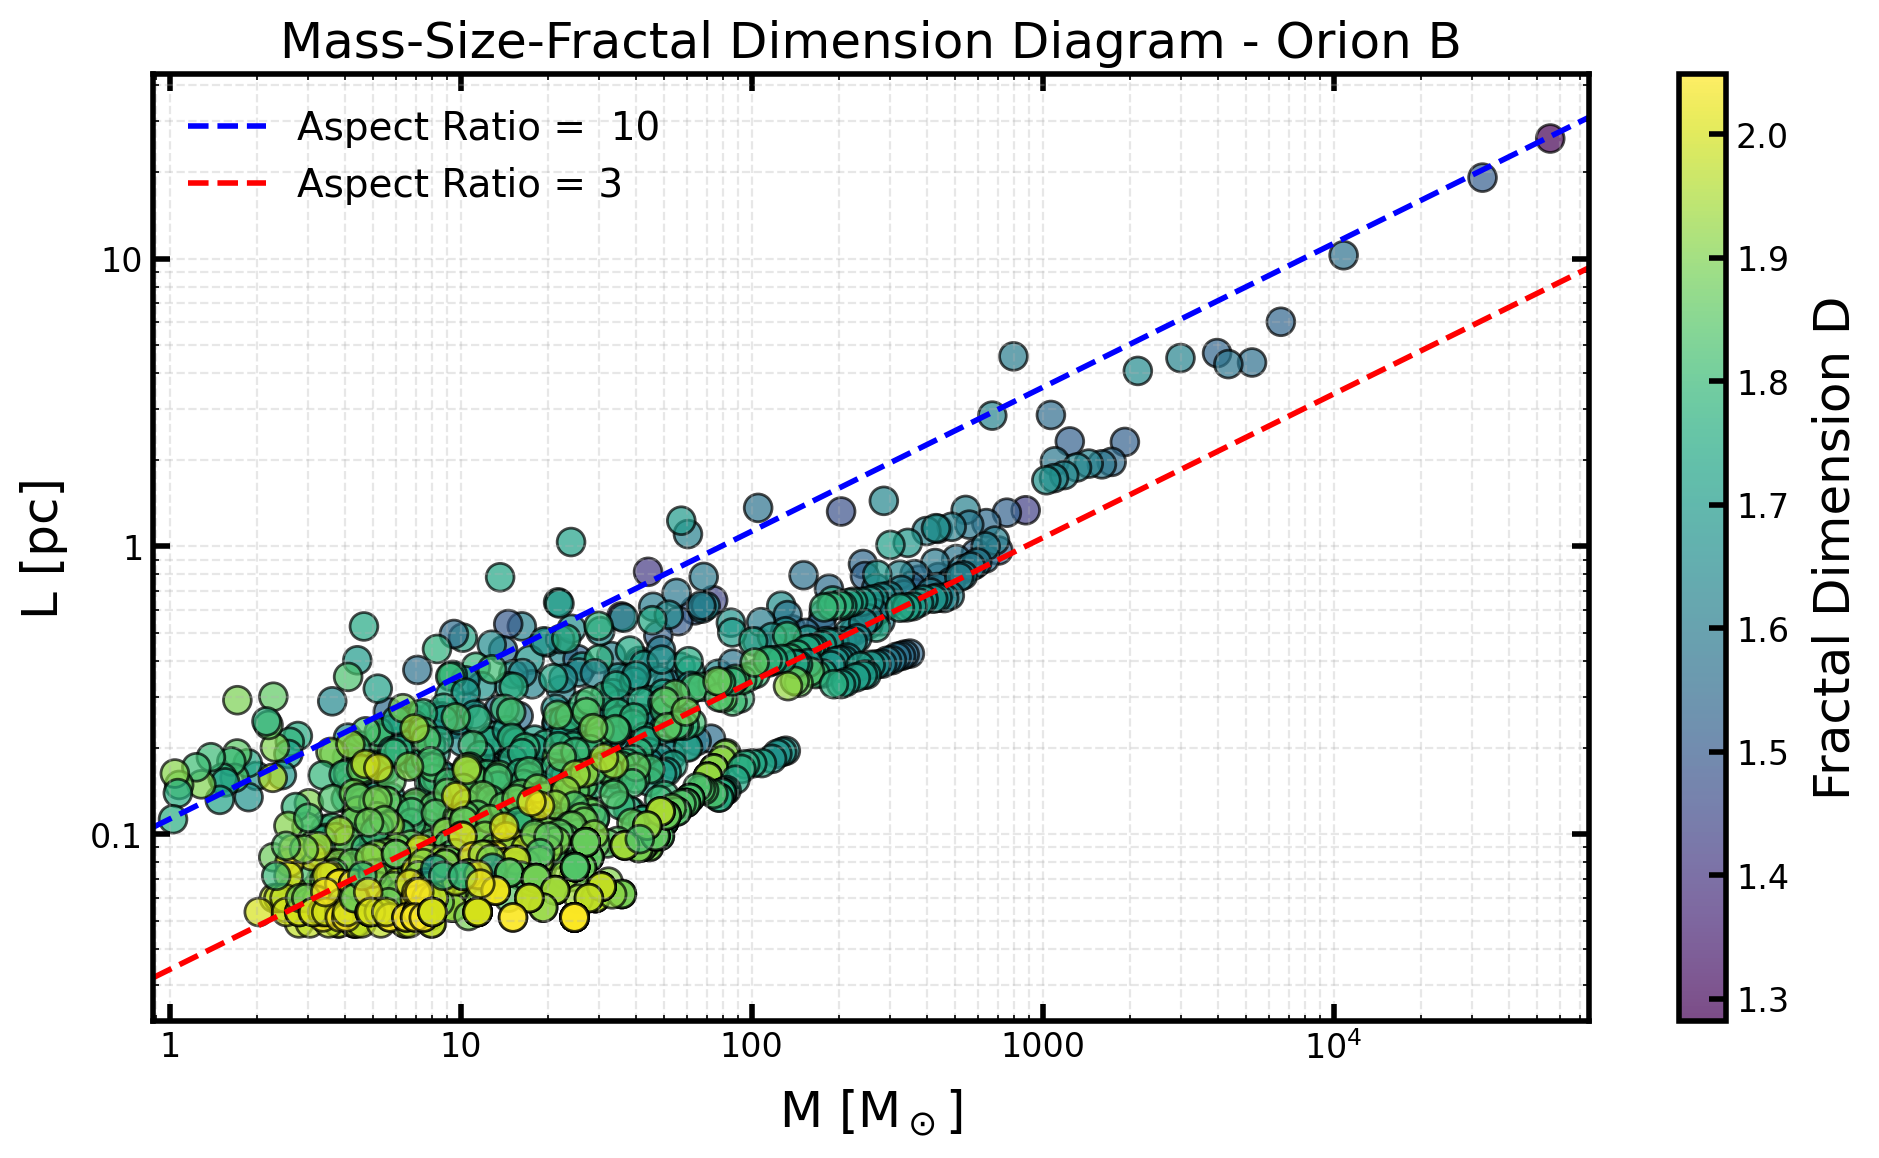
\includegraphics[width=0.6\textwidth]{figures/MSD_Orion_B.png}
    \caption{MSD plane for Orion~B, with color coding and reference scalings.}
    \label{fig:MSD_orion_B}
\end{figure}

\begin{figure}[t]
    \centering
    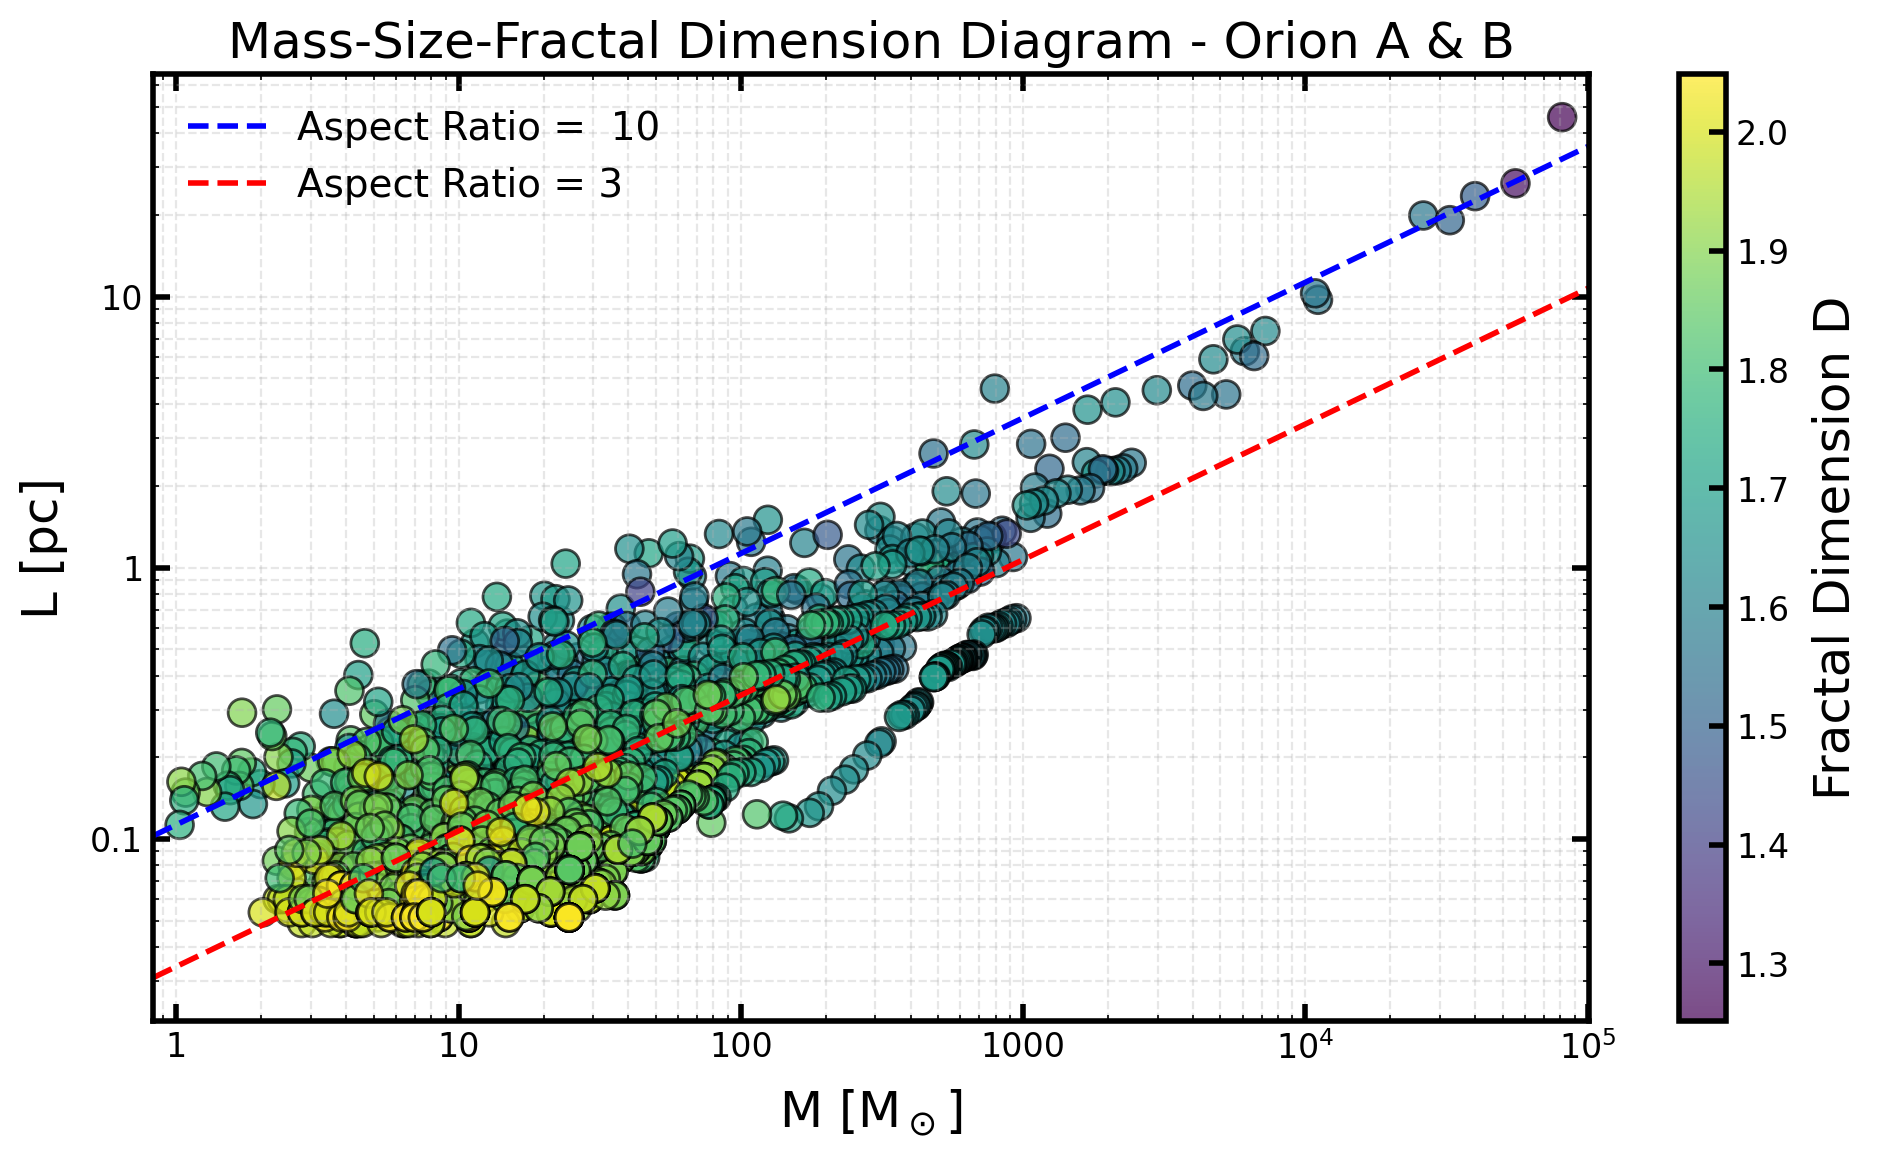
\includegraphics[width=0.6\textwidth]{figures/MSD_Orion_A_B.png}
    \caption{MSD plane for Orion~A and Orion~B combined. The color bar covers the full range of local fractal dimensions across both clouds.}
    \label{fig:MSD_orion_A_B}
\end{figure}

Using this information, we generated spatial maps of the local fractal dimension by assigning to each pixel the value associated with the structure it belongs to.  
If multiple structures overlap, we averaged their values.  
Because of this averaging, the highest values appear slightly reduced compared to the peak values in the previous plots.  
Nevertheless, the maps in Figures~\ref{fig:local_A_map} and~\ref{fig:local_B_map} reinforce the trends already identified in the MSD analysis.

\begin{figure}[t]
    \centering
    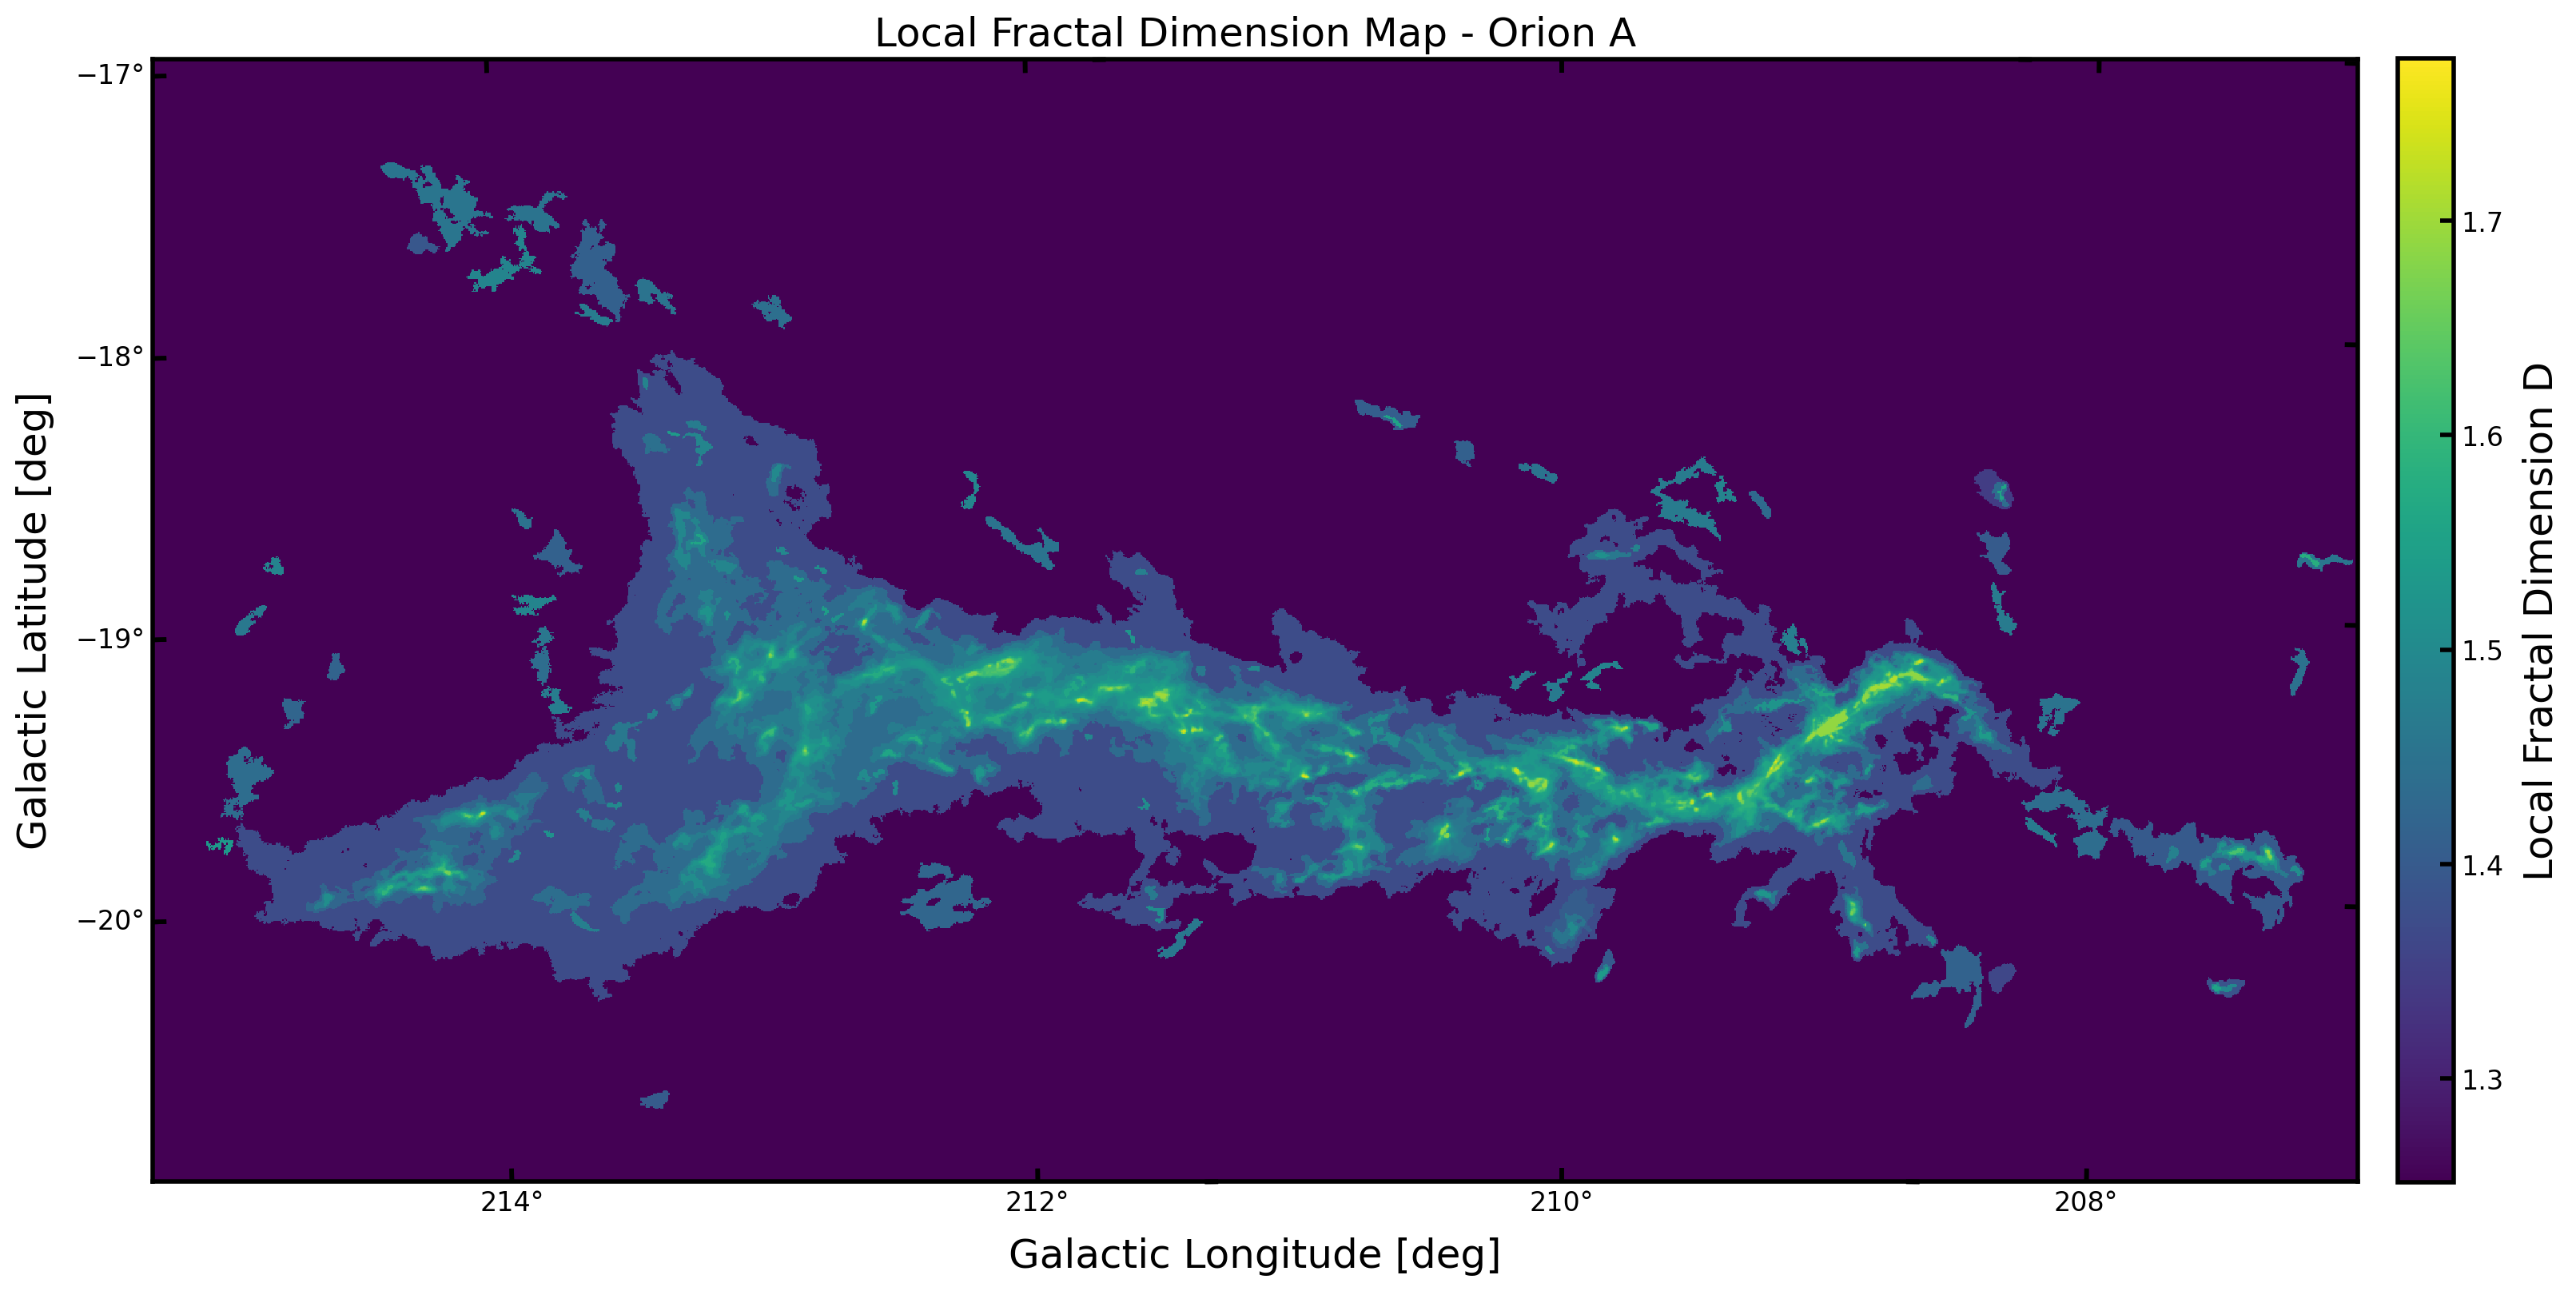
\includegraphics[width=0.75\textwidth]{figures/local_fractal_dimension_map_Orion_A.png}
    \caption{Spatial map of the local fractal dimension for Orion~A. Pixels without assigned structures (NaN) are set to the minimum value of the local fractal dimension.}
    \label{fig:local_A_map}
\end{figure}

% to-do:
% remove the straight lines 
\begin{figure}[t]
    \centering
    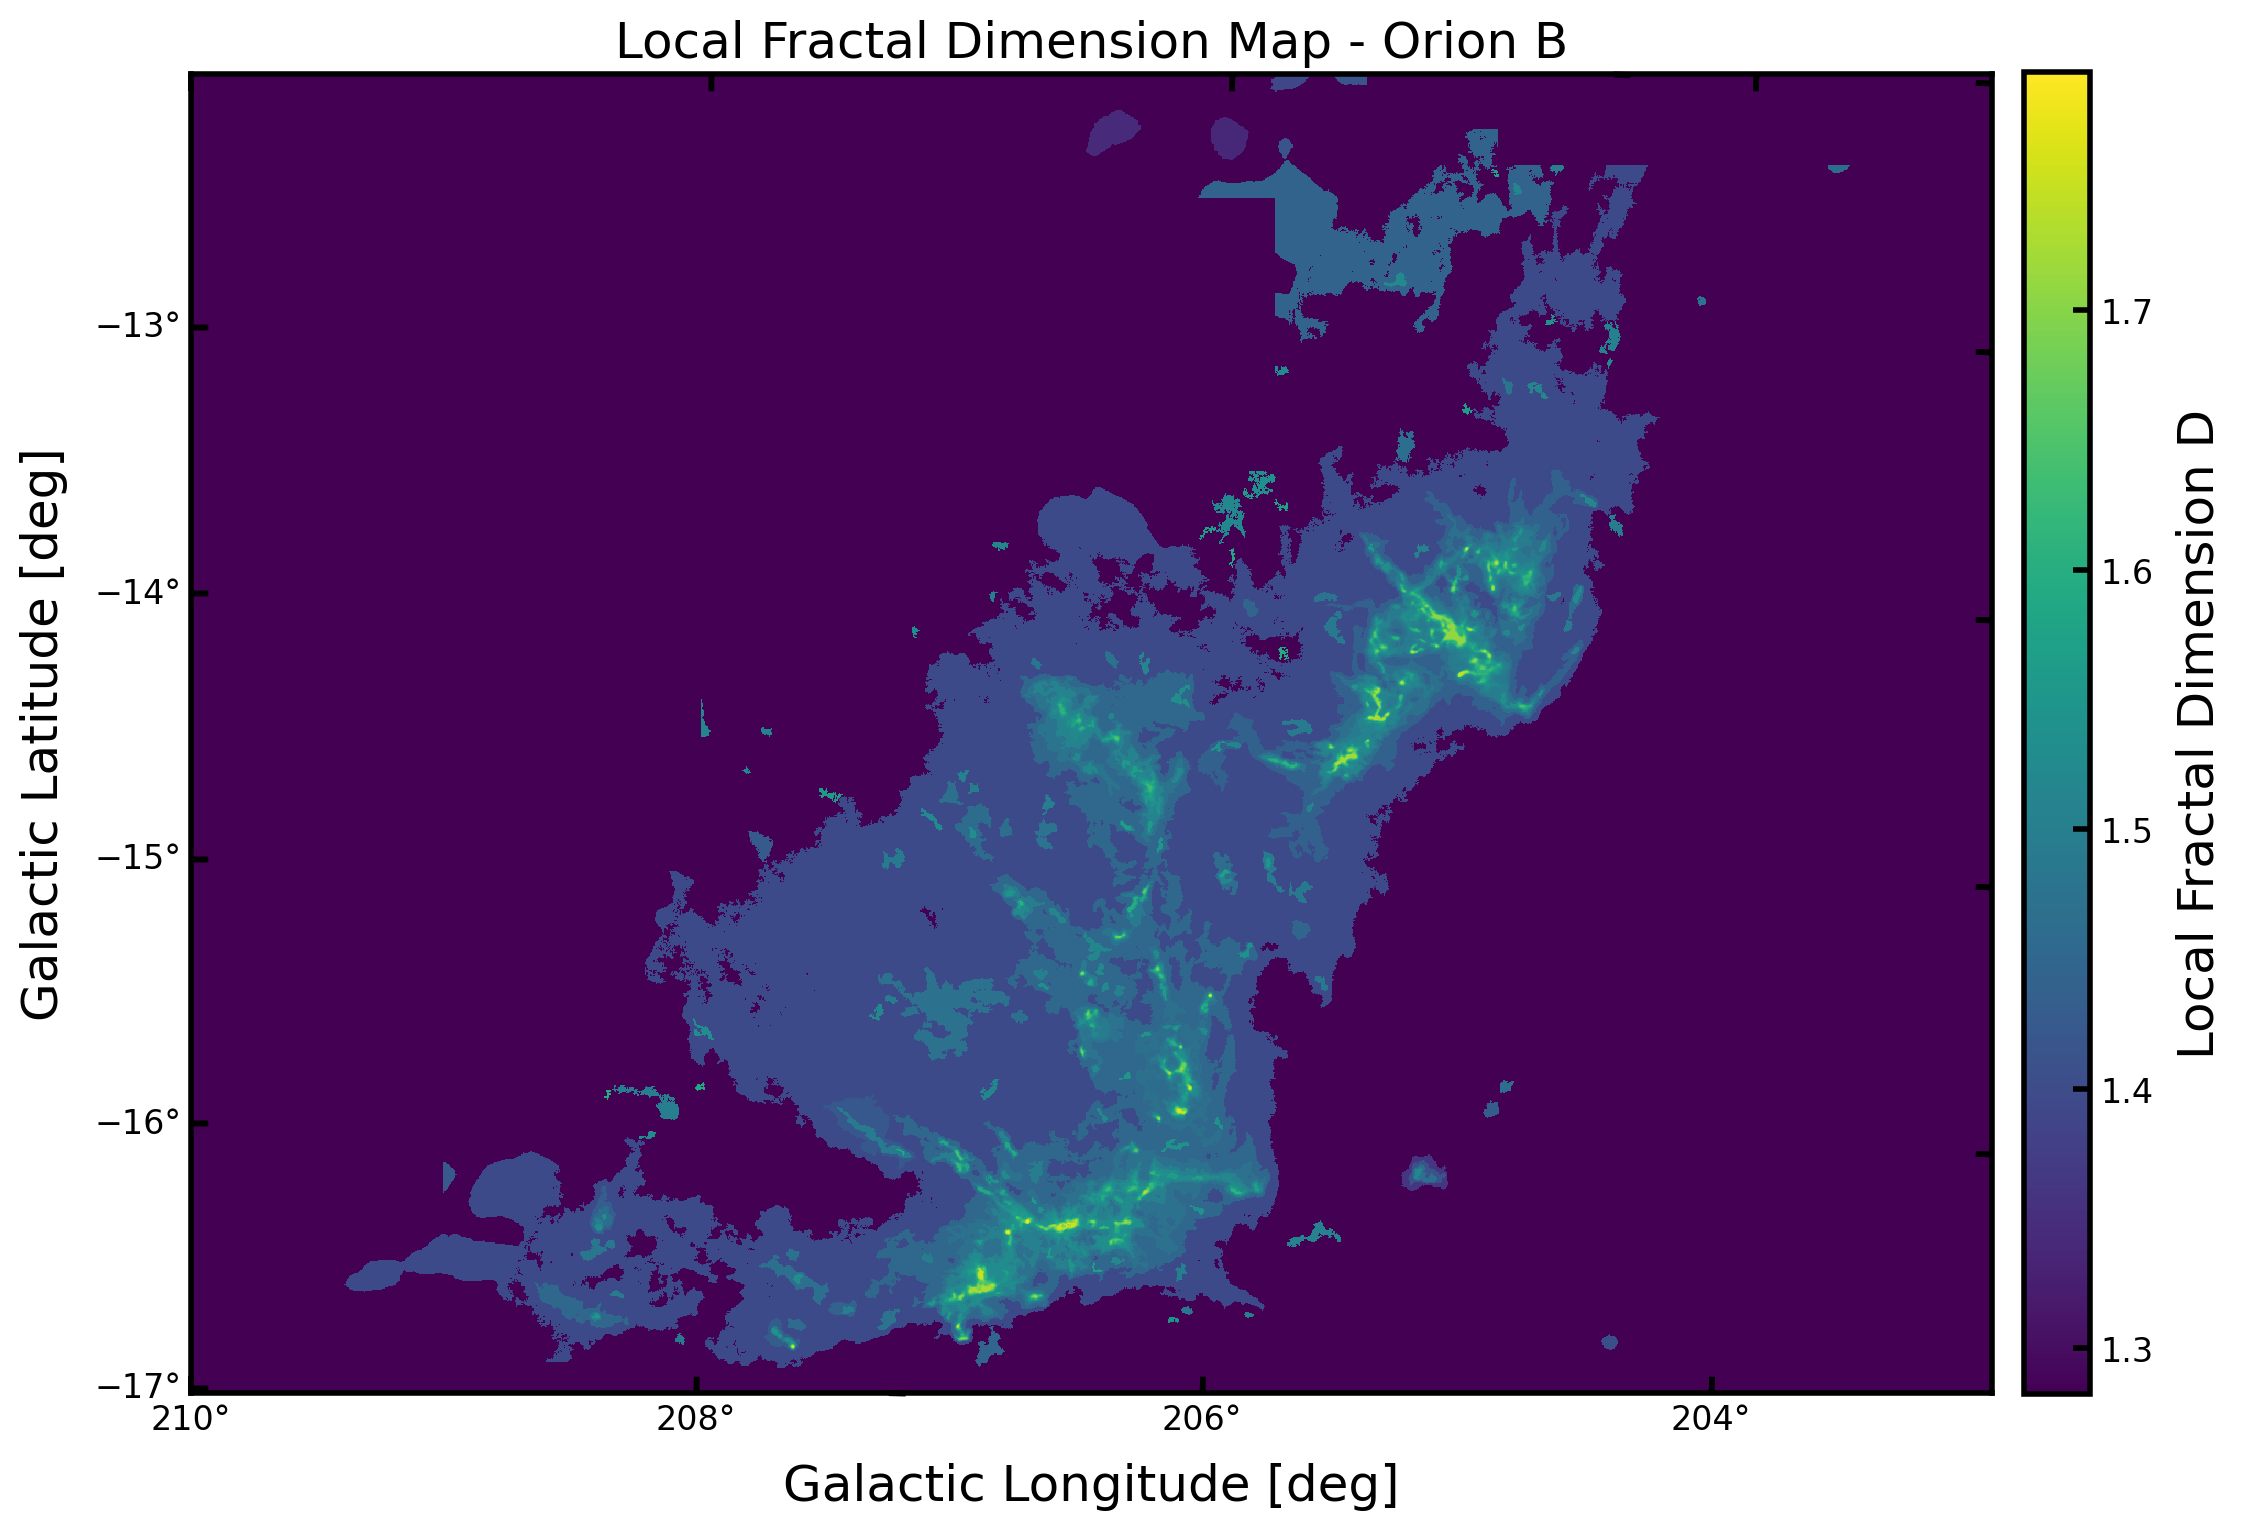
\includegraphics[width=0.6\textwidth]{figures/local_fractal_dimension_map_Orion_B.png}
    \caption{Spatial map of the local fractal dimension for Orion~B. Pixels without assigned structures (NaN) are set to the minimum value of the local fractal dimension.}
    \label{fig:local_B_map}
\end{figure}

An interactive 3D version of the MSD plane is available online at:  
\href{https://simonesped.github.io/MSD_Viz/}{\texttt{MSD 3D Visualizer}}.

Finally, the hierarchical relationships extracted from the dendrogram allow us to track how individual structures break down into substructures.  
This information is visualized in Figures~\ref{fig:MSD_orion_A_lines} and~\ref{fig:MSD_orion_B_lines} in the Appendix, where lines connect each structure to its parent and child structures in the MSD plane.

\section{Connection to Star Formation}

Regions of higher gas density are more conducive to star formation.
To explore this connection, we compared the spatial distribution of the local fractal dimension with the surface density of young stellar objects (YSOs).  
The YSO density maps were obtained by smoothing the distribution of identified YSOs across each region; details of the map construction are provided in the Appendix (Figures \ref{fig:YSOs_density_Map_A}, \ref{fig:YSOs_density_Map_B} for the full sample, Figures \ref{fig:YSOs_density_Map_A_early_stages} and \ref{fig:YSOs_density_Map_B_early_stages}).  
The spatial coverage is naturally limited by the footprint of the available YSO catalog.

We first restricted the analysis to the subset of YSOs classified as early-stage (Class~I and flat-spectrum), which are most likely to be physically associated with ongoing star formation.  
In Orion~A this subset contains 426 objects, while in Orion~B it contains 111.  
Using this subset, the pixel-by-pixel comparison between the YSO density maps and the local fractal dimension yields:
\[
\text{Orion A: Pearson } 0.434, \qquad \text{Spearman } 0.429,
\]
\[
\text{Orion B: Pearson } 0.288, \qquad \text{Spearman } 0.244.
\]

For comparison, we also performed the same analysis using the full YSO sample, without filtering by evolutionary stage.  
The full catalog contains 2818 YSOs in Orion~A and 632 in Orion~B.  
The corresponding correlation coefficients are:
\[
\text{Orion A: Pearson } 0.286, \qquad \text{Spearman } 0.393,
\]
\[
\text{Orion B: Pearson } 0.399, \qquad \text{Spearman } 0.340.
\]

Although the correlations are moderate in both cases, the higher values obtained for the young subset in Orion~A indicate a stronger spatial link between regions of high local fractal dimension and active star formation.  
This supports the interpretation that complex, self-similar structures within the molecular cloud preferentially host the earliest stages of star formation.

% not a lot of pictures here, rather Appendix
\section{Simulations and Uncertainties}

\subsection{Simulations on Global Properties}

\subsubsection{On the Global Fractal Dimension}

To validate the interpretation of the global fractal dimension framework, we performed a series of controlled tests.  
These tests involved applying the fitting routine to mock structures: some were constructed to exhibit a characteristic scale, while others were explicitly scale-free and therefore self-similar.  
As outlined earlier, the method is expected to return a robust and consistent fit only in the absence of a characteristic scale, which would indicate self-similarity.

We first carried out tests on simple geometric figures, in order to confirm the intuition that shapes with simple borders have in this framework a global fractal dimension of 1, and this increase more and more the more complex the boundaries of the shape become. These tests confirmed these expectations.

We then carried out tests on Gaussian Random Fields (GRFs), exploring both GRFs with power-law spectra (scale-free) and GRFs with peaked spectra (dominated by a characteristic scale).  
The simulations consistently confirmed our expectations, showing that the fitting procedure yields more stable and reliable results in the scale-free case, while deviations appear when a characteristic scale is introduced.

We also tested the impact of resolution effects by smoothing the original data with Gaussian kernels of increasing size.  
Even under extreme smoothing, the resulting global fractal dimension varied by no more than -20\,\% relative to the unsmoothed case, indicating that the method is robust within typical observational resolutions. The -20\,\% is also relative to an extreme smoothing case (see Figure \ref{fig:sims_res_global} in the Appendix).

\subsection{Simulations on Local Properties}

\subsubsection{On the Euler Characteristic}

To better understand the expected behavior of the Euler characteristic when applied to real data, we performed dedicated simulations.  
As in the previous tests, the main inputs were Gaussian Random Fields (GRFs), chosen for their well-defined statistical properties and the expectation of a symmetric response.  

The simulations confirmed this expectation: the Euler characteristic exhibits a symmetric profile as a function of the threshold, with a clear maximum in connectivity at the central peak and a gradual decrease on either side.  
This behavior closely resembles a Gaussian bell curve, providing a useful reference pattern for interpreting the results from the actual cloud data.

\subsubsection{On the Local Fractal Dimension}

This section validates the inversion of the perimeter–area (PA) relation and explains how the resulting local fractal dimension should be interpreted in terms of boundary complexity.

We first tested the method on simple, well-understood shapes—straight lines, circles, and Gaussian profiles.  
In these cases it was sometimes necessary to account for the intercept in the original perimeter–area relation (Equation~\ref{eq:perimeter_area}).  
The results were consistent with expectations: lines yielded a dimension of \(D = 2\), simple boxes and circles gave \(D = 1\), and more intricate shapes produced values in between.

We then extended the tests to more complex structures, in particular Gaussian Random Fields (GRFs), to explore how the method behaves in realistic, irregular patterns.  
These experiments revealed a dichotomy that can be described as “sausage vs. hairy caterpillar”:
\begin{itemize}
    \item \textbf{Smooth, compact structures ("sausages")} tend toward \(D(\nu) \approx 2\) in the local PA framework. Their borders are long and coherent with minimal roughness, resulting in a perimeter that scales almost linearly with area.
    \item \textbf{Irregular, space-filling structures ("hairy caterpillars")} tend toward \(D(\nu) \approx 1\). Their boundaries are highly convoluted and expand more slowly with area, leading to a sublinear perimeter–area relationship.
\end{itemize}

A gallery of visual examples illustrating this behavior is provided in the Appendix, and the trends are evident in the observational results (see, for example, Figure~\ref{fig:MSD_orion_A_B}).  
In practice, small and relatively round structures exhibit local fractal dimensions close to 2, whereas larger, more complex structures trend toward 1.

Finally, we examined the effect of resolution on the local fractal dimension using a procedure similar to that employed for the global dimension.  
Smoothing the data with a Gaussian kernel generally reduced the local fractal dimension at most scales.  
At the same time, because the smoothing lowers the highest column-density peaks, the usable column-density range for the analysis becomes narrower.  
This leads to the earlier appearance of artifacts in the PA relation, as documented in the Appendix in Figure \ref{fig:sims_res_local}.

\subsection{Error Estimates}

The uncertainties on the perimeter and area measurements, derived from the simulation procedures described above, are on average approximately 1.6\% for each quantity.  
These uncertainties arise primarily from pixelation effects and the finite resolution of the column–density maps.

An example of the resulting error distributions from a representative simulation is shown in Figure~\ref{fig:uncertainties} in the Appendix.  
The narrow spread around the mean demonstrates that the uncertainty estimates are robust, and that systematic errors remain small compared to the overall dynamic range of the measurements.

\subsection{Comparison with Alternative Methods}

A clear anti-correlation is found when comparing our results with those obtained using the box-counting method, both for the global and the local estimates of the fractal dimension.  
This systematic offset highlights an important scaling dependence: different techniques for quantifying fractal characteristics do not yield directly comparable numerical values.  
Such differences should therefore be carefully considered when interpreting results across studies that adopt different methodological frameworks.
